\documentclass[twoside]{book}

% Packages required by doxygen
\usepackage{calc}
\usepackage{doxygen}
\usepackage{graphicx}
\usepackage[utf8]{inputenc}
\usepackage{makeidx}
\usepackage{multicol}
\usepackage{multirow}
\usepackage{fixltx2e}
\PassOptionsToPackage{warn}{textcomp}
\usepackage{textcomp}
\usepackage[nointegrals]{wasysym}
\usepackage[table]{xcolor}

% Font selection
\usepackage[T1]{fontenc}
\usepackage{mathptmx}
\usepackage[scaled=.90]{helvet}
\usepackage{courier}
\usepackage{amssymb}
\usepackage{sectsty}
\renewcommand{\familydefault}{\sfdefault}
\allsectionsfont{%
  \fontseries{bc}\selectfont%
  \color{darkgray}%
}
\renewcommand{\DoxyLabelFont}{%
  \fontseries{bc}\selectfont%
  \color{darkgray}%
}
\newcommand{\+}{\discretionary{\mbox{\scriptsize$\hookleftarrow$}}{}{}}

% Page & text layout
\usepackage{geometry}
\geometry{%
  a4paper,%
  top=2.5cm,%
  bottom=2.5cm,%
  left=2.5cm,%
  right=2.5cm%
}
\tolerance=750
\hfuzz=15pt
\hbadness=750
\setlength{\emergencystretch}{15pt}
\setlength{\parindent}{0cm}
\setlength{\parskip}{0.2cm}
\makeatletter
\renewcommand{\paragraph}{%
  \@startsection{paragraph}{4}{0ex}{-1.0ex}{1.0ex}{%
    \normalfont\normalsize\bfseries\SS@parafont%
  }%
}
\renewcommand{\subparagraph}{%
  \@startsection{subparagraph}{5}{0ex}{-1.0ex}{1.0ex}{%
    \normalfont\normalsize\bfseries\SS@subparafont%
  }%
}
\makeatother

% Headers & footers
\usepackage{fancyhdr}
\pagestyle{fancyplain}
\fancyhead[LE]{\fancyplain{}{\bfseries\thepage}}
\fancyhead[CE]{\fancyplain{}{}}
\fancyhead[RE]{\fancyplain{}{\bfseries\leftmark}}
\fancyhead[LO]{\fancyplain{}{\bfseries\rightmark}}
\fancyhead[CO]{\fancyplain{}{}}
\fancyhead[RO]{\fancyplain{}{\bfseries\thepage}}
\fancyfoot[LE]{\fancyplain{}{}}
\fancyfoot[CE]{\fancyplain{}{}}
\fancyfoot[RE]{\fancyplain{}{\bfseries\scriptsize Generated on Sun Jun 1 2014 15\+:02\+:16 for I\+N\+F\+O3220 Assignment by Doxygen }}
\fancyfoot[LO]{\fancyplain{}{\bfseries\scriptsize Generated on Sun Jun 1 2014 15\+:02\+:16 for I\+N\+F\+O3220 Assignment by Doxygen }}
\fancyfoot[CO]{\fancyplain{}{}}
\fancyfoot[RO]{\fancyplain{}{}}
\renewcommand{\footrulewidth}{0.4pt}
\renewcommand{\chaptermark}[1]{%
  \markboth{#1}{}%
}
\renewcommand{\sectionmark}[1]{%
  \markright{\thesection\ #1}%
}

% Indices & bibliography
\usepackage{natbib}
\usepackage[titles]{tocloft}
\setcounter{tocdepth}{3}
\setcounter{secnumdepth}{5}
\makeindex

% Hyperlinks (required, but should be loaded last)
\usepackage{ifpdf}
\ifpdf
  \usepackage[pdftex,pagebackref=true]{hyperref}
\else
  \usepackage[ps2pdf,pagebackref=true]{hyperref}
\fi
\hypersetup{%
  colorlinks=true,%
  linkcolor=blue,%
  citecolor=blue,%
  unicode%
}

% Custom commands
\newcommand{\clearemptydoublepage}{%
  \newpage{\pagestyle{empty}\cleardoublepage}%
}


%===== C O N T E N T S =====

\begin{document}

% Titlepage & ToC
\hypersetup{pageanchor=false,
             bookmarks=true,
             bookmarksnumbered=true,
             pdfencoding=unicode
            }
\pagenumbering{roman}
\begin{titlepage}
\vspace*{7cm}
\begin{center}%
{\Large I\+N\+F\+O3220 Assignment \\[1ex]\large 3 }\\
\vspace*{1cm}
{\large Generated by Doxygen 1.8.7}\\
\vspace*{0.5cm}
{\small Sun Jun 1 2014 15:02:16}\\
\end{center}
\end{titlepage}
\clearemptydoublepage
\tableofcontents
\clearemptydoublepage
\pagenumbering{arabic}
\hypersetup{pageanchor=true}

%--- Begin generated contents ---
\chapter{I\+N\+F\+O3220 Assignment Stage 3 Documentation}
\label{index}\hypertarget{index}{}\section*{Changes to Stage 3 code }

In order to extend the code into Stage 3 I had to make some changes to the existing code.

\subsection*{\hyperlink{class_config_reader}{Config\+Reader} }

The \hyperlink{class_config_reader}{Config\+Reader} class was extended to accomodate for additional variables in the configuration file.

\subsection*{Ball-\/\+Brick Collision Bug }

I discovered that the collision logic in the base code was incorrect as it was not detecting the correct sides. If the ball its the top of the brick is will continue to go through the brick, the brick would lose all its life in one hit. To fix this, I had to rewrite their collision logic.

\subsection*{Box Size Bug }

There was a bug where the box width and height were mixed up. This was fixed.

\section*{Design Pattern }

I chose to use the Strategy Design Pattern. This can be seen in the \hyperlink{class_power_up}{Power\+Up}, \hyperlink{class_ball_power_bonus}{Ball\+Power\+Bonus}, \hyperlink{class_ball_size_bonus}{Ball\+Size\+Bonus} and \hyperlink{class_extra_life}{Extra\+Life} classes.

\section*{Extension }

For the extension, I implemented Power\+Ups and Levels.

Power\+Ups will give the ball more size or power. There is also an extra life powerup.

Levels are generated randomly based on the current level. More bricks are generated as the player gets to a higher level.

These extensions can be switched off and on. 
\chapter{Changes to Stage 1 code}
\label{md___users_khanh__i_n_f_o3220__assignment__assignment_three_base_two__r_e_a_d_m_e}
\hypertarget{md___users_khanh__i_n_f_o3220__assignment__assignment_three_base_two__r_e_a_d_m_e}{}
In order to extend the code into Stage 2 I had to make some changes to the existing code.

\subsection*{\hyperlink{class_ball}{Ball} }

The original \hyperlink{class_ball}{Ball} class was renamed \hyperlink{classas1_ball}{as1\+Ball}. This was changed to allow the definition of a new \hyperlink{class_ball}{Ball} class which acts as an adapter to allows \hyperlink{classas1_ball}{as1\+Ball} to be used as a Q\+Graphics\+Item.

\subsection*{\hyperlink{class_config_reader}{Config\+Reader} }

The \hyperlink{class_config_reader}{Config\+Reader} class was extended to accomodate for additional variables in the configuration file.

\subsection*{Dialog }

The functionality of the original Dialog class has been replaced with \hyperlink{class_table_scene}{Table\+Scene} and \hyperlink{class_table_view}{Table\+View} classes which subclass Q\+Graphics\+Scene and Q\+Graphics\+View respectively.

\subsection*{\hyperlink{class_coordinate}{Coordinate} }

The coordinate class was modified to get the frame width and height from the configuration file rather than storing this within \hyperlink{class_coordinate}{Coordinate}. An additional constructor was also added for convenience.

\section*{Design decisions }

As mentioned above the \hyperlink{class_ball}{Ball} class acts as an adapter to allow \hyperlink{classas1_ball}{as1\+Ball} to be used as a Q\+Graphics\+Item. \hyperlink{class_ball}{Ball} inherits from both Q\+Graphics\+Item (publicly) and \hyperlink{classas1_ball}{as1\+Ball} (privately), making this a use of the Class Adapter design pattern.

\section*{Extension }

For the extension I implemented regenerating bricks. Any brick that has previously died can reappear randomly. Bricks that reappear are given a random number of lives, and are given a different colour.

The extension is customisable in terms of\+:


\begin{DoxyItemize}
\item The maximum number of lives a regenerated brick can be given
\item The probability (per frame) that a given dead brick can reappear
\item The colour of the regenerated brick
\end{DoxyItemize}

While only previously defined bricks can reappear, bricks can be defined as initially invisible, and these bricks can 'regenerate'.

I also added the number of lives that each brick has to the brick. This feature can be disabled in the config file. 
\chapter{Hierarchical Index}
\section{Class Hierarchy}
This inheritance list is sorted roughly, but not completely, alphabetically\+:\begin{DoxyCompactList}
\item \contentsline{section}{as1\+Ball}{\pageref{classas1_ball}}{}
\begin{DoxyCompactList}
\item \contentsline{section}{Ball}{\pageref{class_ball}}{}
\end{DoxyCompactList}
\item \contentsline{section}{Config\+Reader\+:\+:brick\+Config}{\pageref{struct_config_reader_1_1brick_config}}{}
\item \contentsline{section}{Config\+Reader}{\pageref{class_config_reader}}{}
\item \contentsline{section}{Coordinate}{\pageref{class_coordinate}}{}
\item \contentsline{section}{Level\+Generator}{\pageref{class_level_generator}}{}
\item \contentsline{section}{Player}{\pageref{class_player}}{}
\item Q\+Graphics\+Item\begin{DoxyCompactList}
\item \contentsline{section}{Ball}{\pageref{class_ball}}{}
\end{DoxyCompactList}
\item Q\+Graphics\+Rect\+Item\begin{DoxyCompactList}
\item \contentsline{section}{Brick}{\pageref{class_brick}}{}
\item \contentsline{section}{Overlay\+Object}{\pageref{class_overlay_object}}{}
\item \contentsline{section}{Paddle}{\pageref{class_paddle}}{}
\item \contentsline{section}{Power\+Up}{\pageref{class_power_up}}{}
\begin{DoxyCompactList}
\item \contentsline{section}{Ball\+Power\+Bonus}{\pageref{class_ball_power_bonus}}{}
\item \contentsline{section}{Ball\+Size\+Bonus}{\pageref{class_ball_size_bonus}}{}
\item \contentsline{section}{Extra\+Life}{\pageref{class_extra_life}}{}
\end{DoxyCompactList}
\end{DoxyCompactList}
\item Q\+Graphics\+Scene\begin{DoxyCompactList}
\item \contentsline{section}{Table\+Scene}{\pageref{class_table_scene}}{}
\end{DoxyCompactList}
\item Q\+Graphics\+View\begin{DoxyCompactList}
\item \contentsline{section}{Table\+View}{\pageref{class_table_view}}{}
\end{DoxyCompactList}
\item Q\+Object\begin{DoxyCompactList}
\item \contentsline{section}{Brick}{\pageref{class_brick}}{}
\item \contentsline{section}{Overlay\+Object}{\pageref{class_overlay_object}}{}
\item \contentsline{section}{Power\+Up}{\pageref{class_power_up}}{}
\end{DoxyCompactList}
\end{DoxyCompactList}

\chapter{Class Index}
\section{Class List}
Here are the classes, structs, unions and interfaces with brief descriptions\+:\begin{DoxyCompactList}
\item\contentsline{section}{\hyperlink{classas1_ball}{as1\+Ball} }{\pageref{classas1_ball}}{}
\item\contentsline{section}{\hyperlink{class_ball}{Ball} }{\pageref{class_ball}}{}
\item\contentsline{section}{\hyperlink{class_ball_power_bonus}{Ball\+Power\+Bonus} }{\pageref{class_ball_power_bonus}}{}
\item\contentsline{section}{\hyperlink{class_ball_size_bonus}{Ball\+Size\+Bonus} }{\pageref{class_ball_size_bonus}}{}
\item\contentsline{section}{\hyperlink{class_brick}{Brick} }{\pageref{class_brick}}{}
\item\contentsline{section}{\hyperlink{struct_config_reader_1_1brick_config}{Config\+Reader\+::brick\+Config} }{\pageref{struct_config_reader_1_1brick_config}}{}
\item\contentsline{section}{\hyperlink{class_config_reader}{Config\+Reader} }{\pageref{class_config_reader}}{}
\item\contentsline{section}{\hyperlink{class_coordinate}{Coordinate} }{\pageref{class_coordinate}}{}
\item\contentsline{section}{\hyperlink{class_extra_life}{Extra\+Life} }{\pageref{class_extra_life}}{}
\item\contentsline{section}{\hyperlink{class_level_generator}{Level\+Generator} }{\pageref{class_level_generator}}{}
\item\contentsline{section}{\hyperlink{class_overlay_object}{Overlay\+Object} }{\pageref{class_overlay_object}}{}
\item\contentsline{section}{\hyperlink{class_paddle}{Paddle} }{\pageref{class_paddle}}{}
\item\contentsline{section}{\hyperlink{class_player}{Player} }{\pageref{class_player}}{}
\item\contentsline{section}{\hyperlink{class_power_up}{Power\+Up} }{\pageref{class_power_up}}{}
\item\contentsline{section}{\hyperlink{class_table_scene}{Table\+Scene} }{\pageref{class_table_scene}}{}
\item\contentsline{section}{\hyperlink{class_table_view}{Table\+View} }{\pageref{class_table_view}}{}
\end{DoxyCompactList}

\chapter{Class Documentation}
\hypertarget{classas1_ball}{\section{as1\+Ball Class Reference}
\label{classas1_ball}\index{as1\+Ball@{as1\+Ball}}
}
Inheritance diagram for as1\+Ball\+:\begin{figure}[H]
\begin{center}
\leavevmode
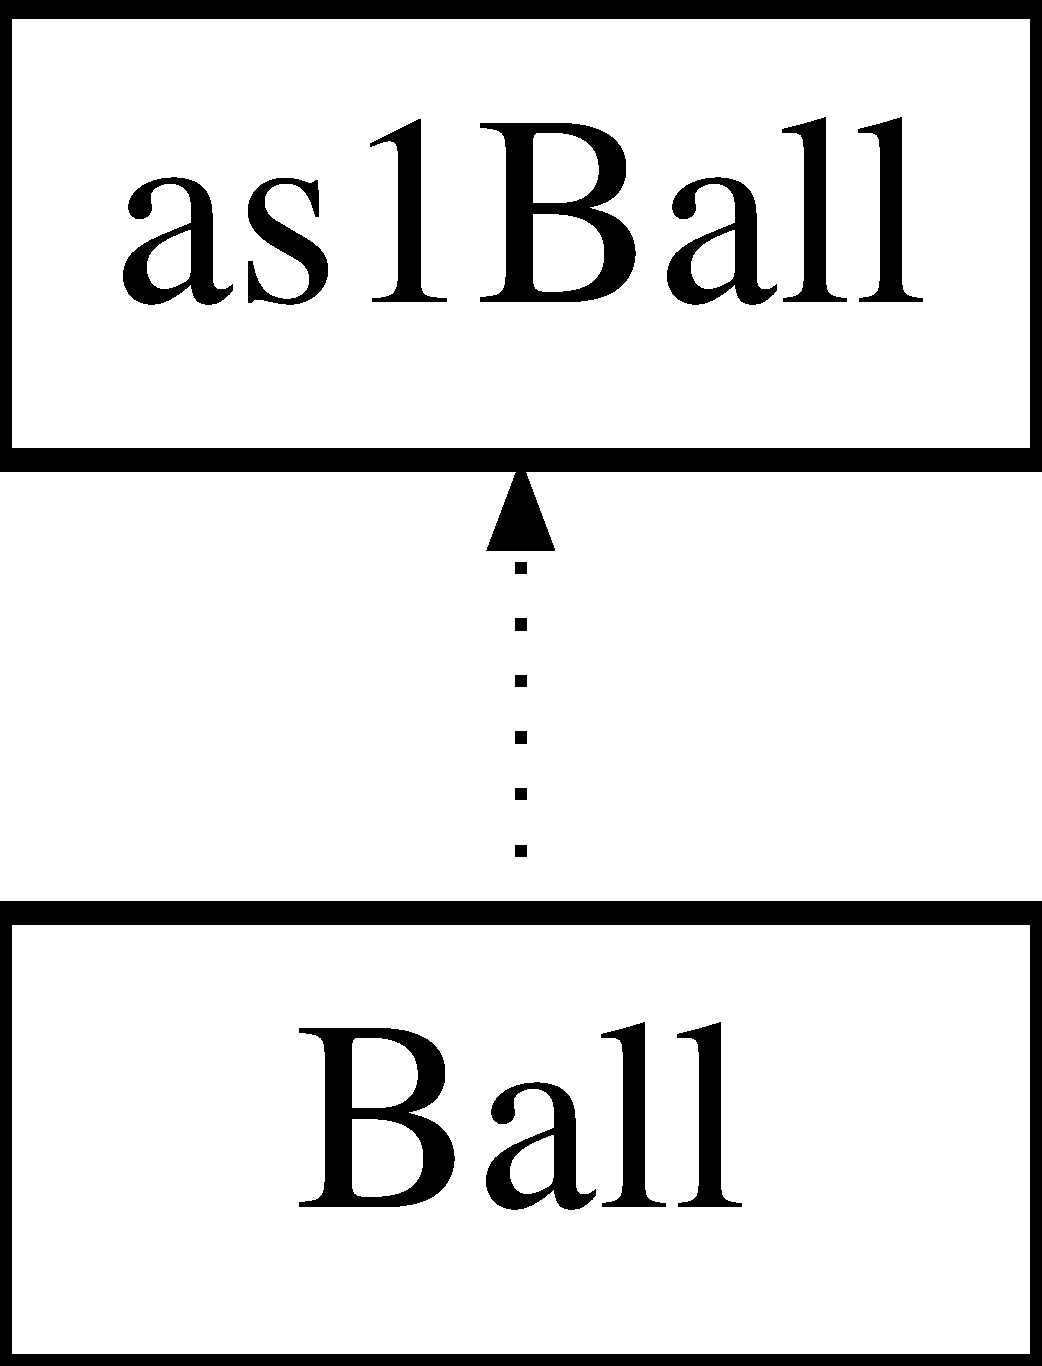
\includegraphics[height=2.000000cm]{classas1_ball}
\end{center}
\end{figure}
\subsection*{Public Member Functions}
\begin{DoxyCompactItemize}
\item 
\hypertarget{classas1_ball_a5871e96a3e1bddf3df7a195688bb06d2}{{\bfseries as1\+Ball} (\hyperlink{class_coordinate}{Coordinate} coordinate)}\label{classas1_ball_a5871e96a3e1bddf3df7a195688bb06d2}

\item 
\hypertarget{classas1_ball_a1c9195b4cb0f4a39fca5d953de5e307b}{{\bfseries as1\+Ball} (\hyperlink{class_coordinate}{Coordinate} coordinate, unsigned int radius)}\label{classas1_ball_a1c9195b4cb0f4a39fca5d953de5e307b}

\item 
\hypertarget{classas1_ball_ad2e4c9d8622aad39d58a4deb53574026}{{\bfseries as1\+Ball} (\hyperlink{class_coordinate}{Coordinate} coordinate, unsigned int radius, double gravity, double x\+Velocity, double y\+Velocity, Q\+Color color=\char`\"{}yellow\char`\"{})}\label{classas1_ball_ad2e4c9d8622aad39d58a4deb53574026}

\item 
\hypertarget{classas1_ball_a8929bd8fd5810527e81608cee0f99bf5}{virtual void {\bfseries load\+Config} ()}\label{classas1_ball_a8929bd8fd5810527e81608cee0f99bf5}

\item 
\hypertarget{classas1_ball_a046852dd2f017ebd18d6ed02abb45528}{virtual void {\bfseries render} (Q\+Painter \&painter, unsigned int time)}\label{classas1_ball_a046852dd2f017ebd18d6ed02abb45528}

\item 
\hypertarget{classas1_ball_aef4912a4fdb0a72b8f29f5d45deb141a}{bool {\bfseries is\+Bottom\+Collision} ()}\label{classas1_ball_aef4912a4fdb0a72b8f29f5d45deb141a}

\item 
\hypertarget{classas1_ball_a20674bb1a8af99b6c51bcde24ba882dc}{bool {\bfseries is\+Ceil\+Collision} ()}\label{classas1_ball_a20674bb1a8af99b6c51bcde24ba882dc}

\item 
\hypertarget{classas1_ball_a5b35c5e1a948dddbe647371e8cf850fe}{bool {\bfseries is\+Left\+Collision} ()}\label{classas1_ball_a5b35c5e1a948dddbe647371e8cf850fe}

\item 
\hypertarget{classas1_ball_aea3ddc6cd7bd1b8aabdee0ccc74e0cbb}{bool {\bfseries is\+Right\+Collision} ()}\label{classas1_ball_aea3ddc6cd7bd1b8aabdee0ccc74e0cbb}

\item 
\hypertarget{classas1_ball_a78df2e2ada3bcfc2c13bea07f624c08a}{virtual unsigned int {\bfseries get\+Radius} ()}\label{classas1_ball_a78df2e2ada3bcfc2c13bea07f624c08a}

\item 
\hypertarget{classas1_ball_ae85073d8c54259c53aef7347d0a1fd8e}{virtual void {\bfseries set\+Radius} (unsigned int radius)}\label{classas1_ball_ae85073d8c54259c53aef7347d0a1fd8e}

\item 
\hypertarget{classas1_ball_ac2a5cb332cccec8c784dd2d44d9b82e0}{virtual Q\+Color {\bfseries get\+Color} () const }\label{classas1_ball_ac2a5cb332cccec8c784dd2d44d9b82e0}

\item 
\hypertarget{classas1_ball_a0c2cffe428baf8d586f05bc229309f64}{virtual void {\bfseries set\+Color} (const Q\+Color \&color)}\label{classas1_ball_a0c2cffe428baf8d586f05bc229309f64}

\item 
\hypertarget{classas1_ball_a4241836c0a915ffce22d4d6ea24d6e12}{\hyperlink{class_coordinate}{Coordinate} {\bfseries coordinate} () const }\label{classas1_ball_a4241836c0a915ffce22d4d6ea24d6e12}

\item 
\hypertarget{classas1_ball_a4ac05af1d90fdda9a93fcd64f9a406c2}{void {\bfseries set\+Coordinate} (const \hyperlink{class_coordinate}{Coordinate} \&coordinate)}\label{classas1_ball_a4ac05af1d90fdda9a93fcd64f9a406c2}

\item 
\hypertarget{classas1_ball_ae81e1f764f335e54d9d84df62b7186e3}{virtual double {\bfseries gravity} () const }\label{classas1_ball_ae81e1f764f335e54d9d84df62b7186e3}

\item 
\hypertarget{classas1_ball_a79a5a810e5d904f97cd69d60718f3db7}{virtual void {\bfseries set\+Gravity} (double gravity)}\label{classas1_ball_a79a5a810e5d904f97cd69d60718f3db7}

\item 
\hypertarget{classas1_ball_a7b3d89540f1d10414108b4b630a8c282}{virtual double {\bfseries x\+Velocity} () const }\label{classas1_ball_a7b3d89540f1d10414108b4b630a8c282}

\item 
\hypertarget{classas1_ball_aa54cf0547ab8368ad8c34f5296bca755}{virtual void {\bfseries set\+X\+Velocity} (double x\+Velocity)}\label{classas1_ball_aa54cf0547ab8368ad8c34f5296bca755}

\item 
\hypertarget{classas1_ball_a7e973374f9b8c41266fa2015a78ab525}{virtual double {\bfseries y\+Velocity} () const }\label{classas1_ball_a7e973374f9b8c41266fa2015a78ab525}

\item 
\hypertarget{classas1_ball_ab616bff9e12c9cc9d0fc1f8c7d4f47ec}{virtual void {\bfseries set\+Y\+Velocity} (double y\+Velocity)}\label{classas1_ball_ab616bff9e12c9cc9d0fc1f8c7d4f47ec}

\end{DoxyCompactItemize}
\subsection*{Protected Attributes}
\begin{DoxyCompactItemize}
\item 
\hypertarget{classas1_ball_aa71097d6b0e160c7cca230730959c753}{\hyperlink{class_coordinate}{Coordinate} {\bfseries m\+\_\+coordinate}}\label{classas1_ball_aa71097d6b0e160c7cca230730959c753}

\item 
\hypertarget{classas1_ball_a033cca501e932a3fcb28063f3d5d3c9d}{unsigned int {\bfseries m\+\_\+radius}}\label{classas1_ball_a033cca501e932a3fcb28063f3d5d3c9d}

\item 
\hypertarget{classas1_ball_a7c46582889cdb5335357b634c2026b89}{double {\bfseries m\+\_\+gravity}}\label{classas1_ball_a7c46582889cdb5335357b634c2026b89}

\item 
\hypertarget{classas1_ball_ad8127f307f5be700ff7ef44e996849b4}{double {\bfseries m\+\_\+x\+Velocity}}\label{classas1_ball_ad8127f307f5be700ff7ef44e996849b4}

\item 
\hypertarget{classas1_ball_afeb0990e9b925a3119fe81ca6fc853d8}{double {\bfseries m\+\_\+y\+Velocity}}\label{classas1_ball_afeb0990e9b925a3119fe81ca6fc853d8}

\item 
\hypertarget{classas1_ball_a7c0dd5d4271acad05eaf659c44819b74}{Q\+Color {\bfseries m\+\_\+color}}\label{classas1_ball_a7c0dd5d4271acad05eaf659c44819b74}

\end{DoxyCompactItemize}


The documentation for this class was generated from the following files\+:\begin{DoxyCompactItemize}
\item 
/\+Users/khanh/\+I\+N\+F\+O3220\+\_\+\+Assignment/\+Assignment\+Three\+Base\+Two/as1ball.\+h\item 
/\+Users/khanh/\+I\+N\+F\+O3220\+\_\+\+Assignment/\+Assignment\+Three\+Base\+Two/as1ball.\+cpp\end{DoxyCompactItemize}

\hypertarget{class_ball}{\section{Ball Class Reference}
\label{class_ball}\index{Ball@{Ball}}
}
Inheritance diagram for Ball\+:\begin{figure}[H]
\begin{center}
\leavevmode
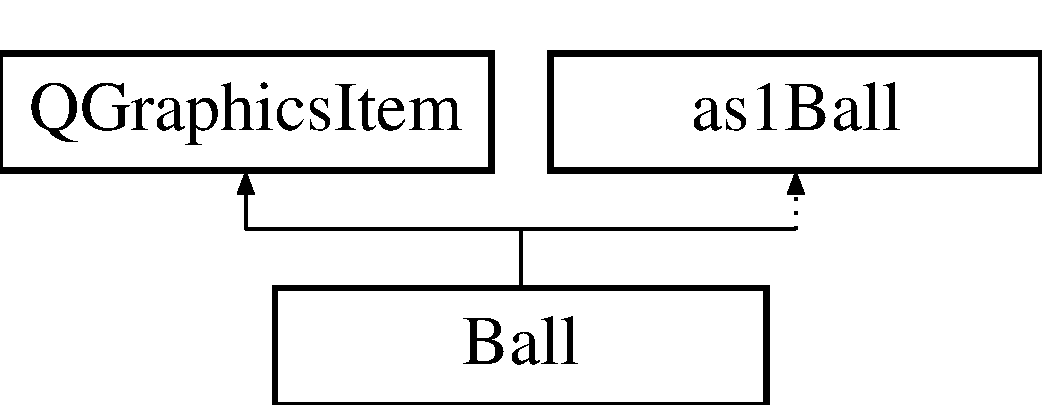
\includegraphics[height=2.000000cm]{class_ball}
\end{center}
\end{figure}
\subsection*{Public Member Functions}
\begin{DoxyCompactItemize}
\item 
\hypertarget{class_ball_a5a588a1c1c218aa5f6d8578801da719a}{{\bfseries Ball} (Q\+Point\+F coordinate, unsigned int radius, double x\+Velocity, double y\+Velocity, Q\+Color color)}\label{class_ball_a5a588a1c1c218aa5f6d8578801da719a}

\item 
\hyperlink{class_ball_acff1695dfbb0dd58a5356efef558182d}{Ball} (const \hyperlink{class_ball}{Ball} \&other)
\begin{DoxyCompactList}\small\item\em \hyperlink{class_ball}{Ball} copy constructor. \end{DoxyCompactList}\item 
bool \hyperlink{class_ball_a2252d47f1db0da83386d82f7b5e59c0f}{is\+Bottom\+Collision} () const 
\begin{DoxyCompactList}\small\item\em Detects whether the ball has hit the bottom of the scene. \end{DoxyCompactList}\item 
bool \hyperlink{class_ball_ab40a04388b295fea9a2e6e682b99bfdc}{is\+Ceil\+Collision} () const 
\begin{DoxyCompactList}\small\item\em Detects whether the ball has hit the top of the scene. \end{DoxyCompactList}\item 
bool \hyperlink{class_ball_a6f691389189d6799de693fbfaf3324e4}{is\+Left\+Collision} () const 
\begin{DoxyCompactList}\small\item\em Detects whether the ball has hit the left side of the scene. \end{DoxyCompactList}\item 
bool \hyperlink{class_ball_a68aa186abe6ef475588bfed3f3eb83de}{is\+Right\+Collision} () const 
\begin{DoxyCompactList}\small\item\em Detects whether the ball has hit the right side of the scene. \end{DoxyCompactList}\item 
\hypertarget{class_ball_aaf64ce0df64b577edaaa677cd8b5b961}{Q\+Point\+F {\bfseries coordinate} () const }\label{class_ball_aaf64ce0df64b577edaaa677cd8b5b961}

\item 
void \hyperlink{class_ball_a69b5819e8b0b441f0412762ab2e0e3db}{set\+Coordinate} (const Q\+Point\+F \&coordinate)
\begin{DoxyCompactList}\small\item\em Sets coordinate of the ball. \end{DoxyCompactList}\item 
int \hyperlink{class_ball_a075ae9c0cb4d07a368aab11538196657}{get\+Power} ()
\begin{DoxyCompactList}\small\item\em Returns the power of the ball. \end{DoxyCompactList}\item 
int \hyperlink{class_ball_a7915b97921a5aeb5885988689de34306}{set\+Power} (int new\+Power)
\begin{DoxyCompactList}\small\item\em Sets the power of the ball. \end{DoxyCompactList}\item 
void \hyperlink{class_ball_a01c8296409b7ab1a4656bdaf69a8d792}{restore\+Default\+Radius} ()
\begin{DoxyCompactList}\small\item\em Sets the radius to the default radius set at initialisation. \end{DoxyCompactList}\end{DoxyCompactItemize}
\subsection*{Protected Member Functions}
\begin{DoxyCompactItemize}
\item 
virtual void \hyperlink{class_ball_a8eef85bb7dc74d73796c8255e296a758}{advance} (int step)
\begin{DoxyCompactList}\small\item\em Sets the state of the ball as the frame of the scene is advancing. \end{DoxyCompactList}\item 
virtual Q\+Rect\+F \hyperlink{class_ball_ae68484e656a6c7a195e41185c06e9e8f}{bounding\+Rect} () const 
\begin{DoxyCompactList}\small\item\em Overloaded Q\+Graphics\+Item\+::bounding\+Rect. \end{DoxyCompactList}\item 
virtual Q\+Painter\+Path \hyperlink{class_ball_abbfd8d6c4f25ee9236ccc49fc68e1efa}{shape} () const 
\begin{DoxyCompactList}\small\item\em Overloaded Q\+Graphics\+Item\+::shape. \end{DoxyCompactList}\item 
virtual void \hyperlink{class_ball_ac61500d8ef7bbb595175da04c323949c}{paint} (Q\+Painter $\ast$painter, const Q\+Style\+Option\+Graphics\+Item $\ast$option, Q\+Widget $\ast$widget)
\begin{DoxyCompactList}\small\item\em Paints the ball object. \end{DoxyCompactList}\end{DoxyCompactItemize}


\subsection{Constructor \& Destructor Documentation}
\hypertarget{class_ball_acff1695dfbb0dd58a5356efef558182d}{\index{Ball@{Ball}!Ball@{Ball}}
\index{Ball@{Ball}!Ball@{Ball}}
\subsubsection[{Ball}]{\setlength{\rightskip}{0pt plus 5cm}Ball\+::\+Ball (
\begin{DoxyParamCaption}
\item[{const {\bf Ball} \&}]{other}
\end{DoxyParamCaption}
)}}\label{class_ball_acff1695dfbb0dd58a5356efef558182d}


\hyperlink{class_ball}{Ball} copy constructor. 

Explict copy constructor as base class 'Q\+Graphics\+Item' has private copy constructor


\begin{DoxyParams}{Parameters}
{\em other} & The object to copy to \\
\hline
\end{DoxyParams}


\subsection{Member Function Documentation}
\hypertarget{class_ball_a8eef85bb7dc74d73796c8255e296a758}{\index{Ball@{Ball}!advance@{advance}}
\index{advance@{advance}!Ball@{Ball}}
\subsubsection[{advance}]{\setlength{\rightskip}{0pt plus 5cm}void Ball\+::advance (
\begin{DoxyParamCaption}
\item[{int}]{step}
\end{DoxyParamCaption}
)\hspace{0.3cm}{\ttfamily [protected]}, {\ttfamily [virtual]}}}\label{class_ball_a8eef85bb7dc74d73796c8255e296a758}


Sets the state of the ball as the frame of the scene is advancing. 

Called by the advance method of the parent Table.

This method is called twice. The first time with step == 0 to indicate the scene is about to advance, and a second time with step == 1 to indicate the scene is advancing.


\begin{DoxyParams}{Parameters}
{\em step} & \\
\hline
\end{DoxyParams}
\hypertarget{class_ball_ae68484e656a6c7a195e41185c06e9e8f}{\index{Ball@{Ball}!bounding\+Rect@{bounding\+Rect}}
\index{bounding\+Rect@{bounding\+Rect}!Ball@{Ball}}
\subsubsection[{bounding\+Rect}]{\setlength{\rightskip}{0pt plus 5cm}Q\+Rect\+F Ball\+::bounding\+Rect (
\begin{DoxyParamCaption}
{}
\end{DoxyParamCaption}
) const\hspace{0.3cm}{\ttfamily [protected]}, {\ttfamily [virtual]}}}\label{class_ball_ae68484e656a6c7a195e41185c06e9e8f}


Overloaded Q\+Graphics\+Item\+::bounding\+Rect. 

Defines the approximate size of the object. This is used to determine whether the object requires redrawing in the scene.

\begin{DoxyReturn}{Returns}
Q\+Rect\+F defining the obejct in the local coordinate system 
\end{DoxyReturn}
\hypertarget{class_ball_a075ae9c0cb4d07a368aab11538196657}{\index{Ball@{Ball}!get\+Power@{get\+Power}}
\index{get\+Power@{get\+Power}!Ball@{Ball}}
\subsubsection[{get\+Power}]{\setlength{\rightskip}{0pt plus 5cm}int Ball\+::get\+Power (
\begin{DoxyParamCaption}
{}
\end{DoxyParamCaption}
)}}\label{class_ball_a075ae9c0cb4d07a368aab11538196657}


Returns the power of the ball. 

\begin{DoxyReturn}{Returns}
int 
\end{DoxyReturn}
\hypertarget{class_ball_a2252d47f1db0da83386d82f7b5e59c0f}{\index{Ball@{Ball}!is\+Bottom\+Collision@{is\+Bottom\+Collision}}
\index{is\+Bottom\+Collision@{is\+Bottom\+Collision}!Ball@{Ball}}
\subsubsection[{is\+Bottom\+Collision}]{\setlength{\rightskip}{0pt plus 5cm}bool Ball\+::is\+Bottom\+Collision (
\begin{DoxyParamCaption}
{}
\end{DoxyParamCaption}
) const}}\label{class_ball_a2252d47f1db0da83386d82f7b5e59c0f}


Detects whether the ball has hit the bottom of the scene. 

\begin{DoxyReturn}{Returns}
bool 
\end{DoxyReturn}
\hypertarget{class_ball_ab40a04388b295fea9a2e6e682b99bfdc}{\index{Ball@{Ball}!is\+Ceil\+Collision@{is\+Ceil\+Collision}}
\index{is\+Ceil\+Collision@{is\+Ceil\+Collision}!Ball@{Ball}}
\subsubsection[{is\+Ceil\+Collision}]{\setlength{\rightskip}{0pt plus 5cm}bool Ball\+::is\+Ceil\+Collision (
\begin{DoxyParamCaption}
{}
\end{DoxyParamCaption}
) const}}\label{class_ball_ab40a04388b295fea9a2e6e682b99bfdc}


Detects whether the ball has hit the top of the scene. 

\begin{DoxyReturn}{Returns}
bool 
\end{DoxyReturn}
\hypertarget{class_ball_a6f691389189d6799de693fbfaf3324e4}{\index{Ball@{Ball}!is\+Left\+Collision@{is\+Left\+Collision}}
\index{is\+Left\+Collision@{is\+Left\+Collision}!Ball@{Ball}}
\subsubsection[{is\+Left\+Collision}]{\setlength{\rightskip}{0pt plus 5cm}bool Ball\+::is\+Left\+Collision (
\begin{DoxyParamCaption}
{}
\end{DoxyParamCaption}
) const}}\label{class_ball_a6f691389189d6799de693fbfaf3324e4}


Detects whether the ball has hit the left side of the scene. 

\begin{DoxyReturn}{Returns}
bool 
\end{DoxyReturn}
\hypertarget{class_ball_a68aa186abe6ef475588bfed3f3eb83de}{\index{Ball@{Ball}!is\+Right\+Collision@{is\+Right\+Collision}}
\index{is\+Right\+Collision@{is\+Right\+Collision}!Ball@{Ball}}
\subsubsection[{is\+Right\+Collision}]{\setlength{\rightskip}{0pt plus 5cm}bool Ball\+::is\+Right\+Collision (
\begin{DoxyParamCaption}
{}
\end{DoxyParamCaption}
) const}}\label{class_ball_a68aa186abe6ef475588bfed3f3eb83de}


Detects whether the ball has hit the right side of the scene. 

\begin{DoxyReturn}{Returns}
bool 
\end{DoxyReturn}
\hypertarget{class_ball_ac61500d8ef7bbb595175da04c323949c}{\index{Ball@{Ball}!paint@{paint}}
\index{paint@{paint}!Ball@{Ball}}
\subsubsection[{paint}]{\setlength{\rightskip}{0pt plus 5cm}void Ball\+::paint (
\begin{DoxyParamCaption}
\item[{Q\+Painter $\ast$}]{painter, }
\item[{const Q\+Style\+Option\+Graphics\+Item $\ast$}]{option, }
\item[{Q\+Widget $\ast$}]{widget}
\end{DoxyParamCaption}
)\hspace{0.3cm}{\ttfamily [protected]}, {\ttfamily [virtual]}}}\label{class_ball_ac61500d8ef7bbb595175da04c323949c}


Paints the ball object. 

Performs the painting of the ball in the parent Table object using the given painter.


\begin{DoxyParams}{Parameters}
{\em painter} & in which to perform painting \\
\hline
\end{DoxyParams}
\hypertarget{class_ball_a01c8296409b7ab1a4656bdaf69a8d792}{\index{Ball@{Ball}!restore\+Default\+Radius@{restore\+Default\+Radius}}
\index{restore\+Default\+Radius@{restore\+Default\+Radius}!Ball@{Ball}}
\subsubsection[{restore\+Default\+Radius}]{\setlength{\rightskip}{0pt plus 5cm}void Ball\+::restore\+Default\+Radius (
\begin{DoxyParamCaption}
{}
\end{DoxyParamCaption}
)}}\label{class_ball_a01c8296409b7ab1a4656bdaf69a8d792}


Sets the radius to the default radius set at initialisation. 

\begin{DoxyReturn}{Returns}
void 
\end{DoxyReturn}
\hypertarget{class_ball_a69b5819e8b0b441f0412762ab2e0e3db}{\index{Ball@{Ball}!set\+Coordinate@{set\+Coordinate}}
\index{set\+Coordinate@{set\+Coordinate}!Ball@{Ball}}
\subsubsection[{set\+Coordinate}]{\setlength{\rightskip}{0pt plus 5cm}void Ball\+::set\+Coordinate (
\begin{DoxyParamCaption}
\item[{const Q\+Point\+F \&}]{coordinate}
\end{DoxyParamCaption}
)}}\label{class_ball_a69b5819e8b0b441f0412762ab2e0e3db}


Sets coordinate of the ball. 

Takes in Q\+Point\+F which is a coordinate, and sets it to the \hyperlink{class_ball}{Ball} object


\begin{DoxyParams}{Parameters}
{\em Q\+Point\+F} & coordinate which is the coordinate that the ball will be set to \\
\hline
\end{DoxyParams}
\hypertarget{class_ball_a7915b97921a5aeb5885988689de34306}{\index{Ball@{Ball}!set\+Power@{set\+Power}}
\index{set\+Power@{set\+Power}!Ball@{Ball}}
\subsubsection[{set\+Power}]{\setlength{\rightskip}{0pt plus 5cm}int Ball\+::set\+Power (
\begin{DoxyParamCaption}
\item[{int}]{new\+Power}
\end{DoxyParamCaption}
)}}\label{class_ball_a7915b97921a5aeb5885988689de34306}


Sets the power of the ball. 


\begin{DoxyParams}{Parameters}
{\em int} & value of new power value \\
\hline
\end{DoxyParams}
\begin{DoxyReturn}{Returns}
int value of the new power 
\end{DoxyReturn}
\hypertarget{class_ball_abbfd8d6c4f25ee9236ccc49fc68e1efa}{\index{Ball@{Ball}!shape@{shape}}
\index{shape@{shape}!Ball@{Ball}}
\subsubsection[{shape}]{\setlength{\rightskip}{0pt plus 5cm}Q\+Painter\+Path Ball\+::shape (
\begin{DoxyParamCaption}
{}
\end{DoxyParamCaption}
) const\hspace{0.3cm}{\ttfamily [protected]}, {\ttfamily [virtual]}}}\label{class_ball_abbfd8d6c4f25ee9236ccc49fc68e1efa}


Overloaded Q\+Graphics\+Item\+::shape. 

Defines the detailed size and shape of the object. This is used for collission detection.

\begin{DoxyReturn}{Returns}
Q\+Painter\+Path defining the shape in the local coordinate system 
\end{DoxyReturn}


The documentation for this class was generated from the following files\+:\begin{DoxyCompactItemize}
\item 
/\+Users/khanh/\+I\+N\+F\+O3220\+\_\+\+Assignment/\+Assignment\+Three\+Base\+Two/ball.\+h\item 
/\+Users/khanh/\+I\+N\+F\+O3220\+\_\+\+Assignment/\+Assignment\+Three\+Base\+Two/ball.\+cpp\end{DoxyCompactItemize}

\hypertarget{class_ball_power_bonus}{\section{Ball\+Power\+Bonus Class Reference}
\label{class_ball_power_bonus}\index{Ball\+Power\+Bonus@{Ball\+Power\+Bonus}}
}
Inheritance diagram for Ball\+Power\+Bonus\+:\begin{figure}[H]
\begin{center}
\leavevmode
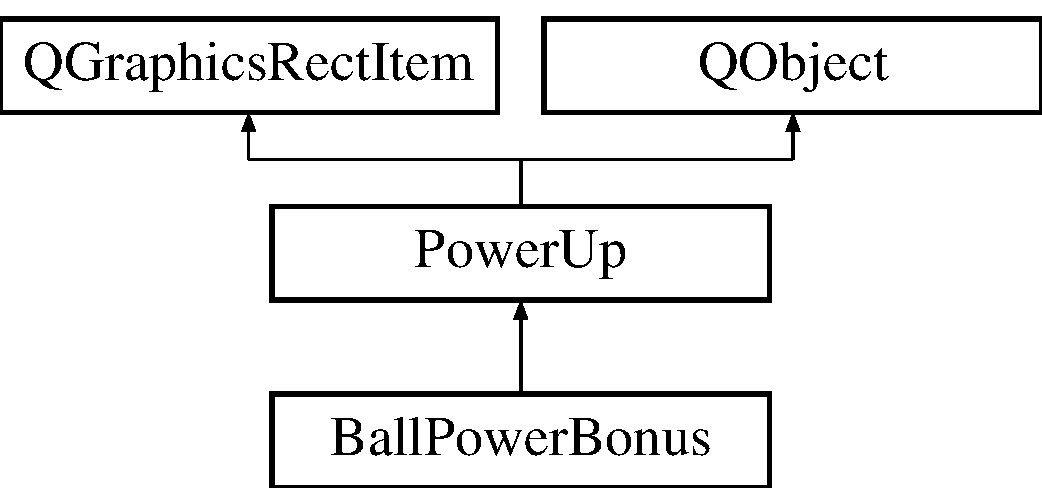
\includegraphics[height=3.000000cm]{class_ball_power_bonus}
\end{center}
\end{figure}
\subsection*{Public Member Functions}
\begin{DoxyCompactItemize}
\item 
\hypertarget{class_ball_power_bonus_a9911fc6afd48931da1fee6cd7a72ab7f}{{\bfseries Ball\+Power\+Bonus} (const Q\+Rect\+F \&rect, Q\+String m\+\_\+title, qreal drop\+Velocity, const Q\+Brush \&fill\+\_\+brush=Q\+Brush())}\label{class_ball_power_bonus_a9911fc6afd48931da1fee6cd7a72ab7f}

\item 
virtual void \hyperlink{class_ball_power_bonus_a842749971fce9228664924706d8e62e1}{apply\+Bonus} ()
\begin{DoxyCompactList}\small\item\em Pure virtual class of the strategy design pattern. \end{DoxyCompactList}\end{DoxyCompactItemize}
\subsection*{Additional Inherited Members}


\subsection{Member Function Documentation}
\hypertarget{class_ball_power_bonus_a842749971fce9228664924706d8e62e1}{\index{Ball\+Power\+Bonus@{Ball\+Power\+Bonus}!apply\+Bonus@{apply\+Bonus}}
\index{apply\+Bonus@{apply\+Bonus}!Ball\+Power\+Bonus@{Ball\+Power\+Bonus}}
\subsubsection[{apply\+Bonus}]{\setlength{\rightskip}{0pt plus 5cm}void Ball\+Power\+Bonus\+::apply\+Bonus (
\begin{DoxyParamCaption}
{}
\end{DoxyParamCaption}
)\hspace{0.3cm}{\ttfamily [virtual]}}}\label{class_ball_power_bonus_a842749971fce9228664924706d8e62e1}


Pure virtual class of the strategy design pattern. 

\begin{DoxyReturn}{Returns}
void 
\end{DoxyReturn}


Implements \hyperlink{class_power_up}{Power\+Up}.



The documentation for this class was generated from the following files\+:\begin{DoxyCompactItemize}
\item 
/\+Users/khanh/\+I\+N\+F\+O3220\+\_\+\+Assignment/\+Assignment\+Three\+Base\+Two/ballpowerbonus.\+h\item 
/\+Users/khanh/\+I\+N\+F\+O3220\+\_\+\+Assignment/\+Assignment\+Three\+Base\+Two/ballpowerbonus.\+cpp\end{DoxyCompactItemize}

\hypertarget{class_ball_size_bonus}{\section{Ball\+Size\+Bonus Class Reference}
\label{class_ball_size_bonus}\index{Ball\+Size\+Bonus@{Ball\+Size\+Bonus}}
}
Inheritance diagram for Ball\+Size\+Bonus\+:\begin{figure}[H]
\begin{center}
\leavevmode
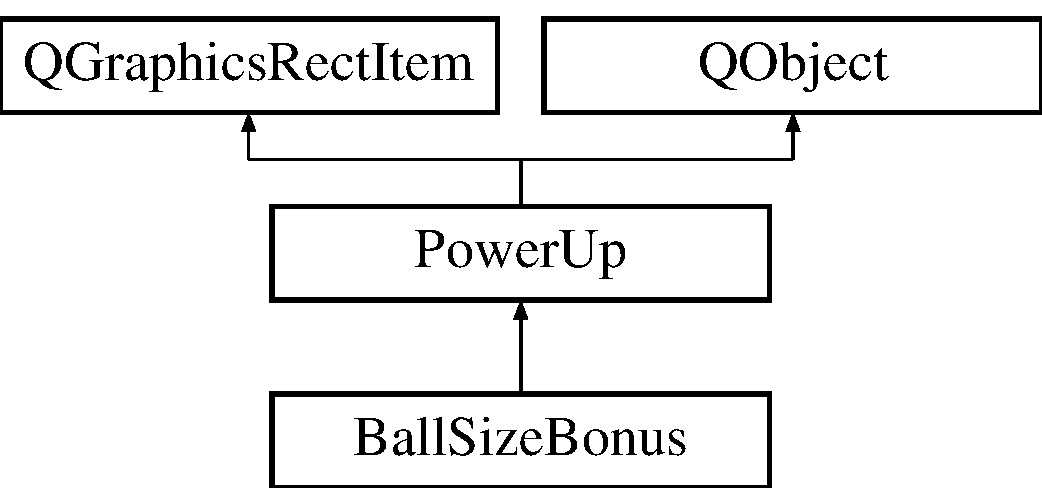
\includegraphics[height=3.000000cm]{class_ball_size_bonus}
\end{center}
\end{figure}
\subsection*{Public Member Functions}
\begin{DoxyCompactItemize}
\item 
\hypertarget{class_ball_size_bonus_adb4ef6b61b0ee2fd6783a2b4dcb91ae4}{{\bfseries Ball\+Size\+Bonus} (const Q\+Rect\+F \&rect, Q\+String m\+\_\+title, qreal drop\+Velocity, const Q\+Brush \&fill\+\_\+brush=Q\+Brush())}\label{class_ball_size_bonus_adb4ef6b61b0ee2fd6783a2b4dcb91ae4}

\item 
virtual void \hyperlink{class_ball_size_bonus_ac780f00fc7ffaeeccb2f93e8a4496ef5}{apply\+Bonus} ()
\begin{DoxyCompactList}\small\item\em Pure virtual class of the strategy design pattern. \end{DoxyCompactList}\end{DoxyCompactItemize}
\subsection*{Additional Inherited Members}


\subsection{Member Function Documentation}
\hypertarget{class_ball_size_bonus_ac780f00fc7ffaeeccb2f93e8a4496ef5}{\index{Ball\+Size\+Bonus@{Ball\+Size\+Bonus}!apply\+Bonus@{apply\+Bonus}}
\index{apply\+Bonus@{apply\+Bonus}!Ball\+Size\+Bonus@{Ball\+Size\+Bonus}}
\subsubsection[{apply\+Bonus}]{\setlength{\rightskip}{0pt plus 5cm}void Ball\+Size\+Bonus\+::apply\+Bonus (
\begin{DoxyParamCaption}
{}
\end{DoxyParamCaption}
)\hspace{0.3cm}{\ttfamily [virtual]}}}\label{class_ball_size_bonus_ac780f00fc7ffaeeccb2f93e8a4496ef5}


Pure virtual class of the strategy design pattern. 

\begin{DoxyReturn}{Returns}
void 
\end{DoxyReturn}


Implements \hyperlink{class_power_up}{Power\+Up}.



The documentation for this class was generated from the following files\+:\begin{DoxyCompactItemize}
\item 
/\+Users/khanh/\+I\+N\+F\+O3220\+\_\+\+Assignment/\+Assignment\+Three\+Base\+Two/ballsizebonus.\+h\item 
/\+Users/khanh/\+I\+N\+F\+O3220\+\_\+\+Assignment/\+Assignment\+Three\+Base\+Two/ballsizebonus.\+cpp\end{DoxyCompactItemize}

\hypertarget{class_brick}{\section{Brick Class Reference}
\label{class_brick}\index{Brick@{Brick}}
}
Inheritance diagram for Brick\+:\begin{figure}[H]
\begin{center}
\leavevmode
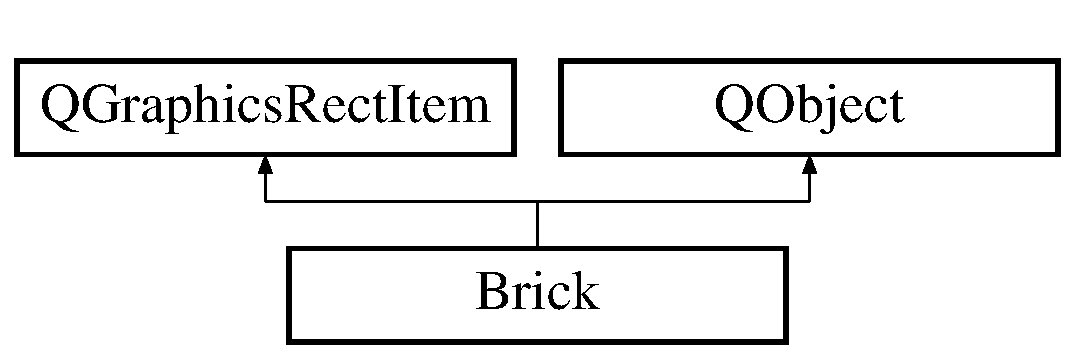
\includegraphics[height=2.000000cm]{class_brick}
\end{center}
\end{figure}
\subsection*{Public Member Functions}
\begin{DoxyCompactItemize}
\item 
\hypertarget{class_brick_a519f7d73685717c8e67532baf4542403}{\hyperlink{class_brick_a519f7d73685717c8e67532baf4542403}{Brick} (const Q\+Rect\+F \&rect, int lives, bool visible, const Q\+Brush \&fill\+\_\+brush=Q\+Brush())}\label{class_brick_a519f7d73685717c8e67532baf4542403}

\begin{DoxyCompactList}\small\item\em \hyperlink{class_brick}{Brick} constructor. \end{DoxyCompactList}\item 
\hyperlink{class_brick_a05b0f571f9d01b963cdf263b2a6c5ce8}{Brick} (const \hyperlink{class_brick}{Brick} \&other)
\begin{DoxyCompactList}\small\item\em \hyperlink{class_brick}{Brick} copy constructor. \end{DoxyCompactList}\item 
\hypertarget{class_brick_adeb99ee821f196f4cb508bf90ef09667}{\hyperlink{class_brick}{Brick} \& \hyperlink{class_brick_adeb99ee821f196f4cb508bf90ef09667}{set\+Num\+Lives} (int lives)}\label{class_brick_adeb99ee821f196f4cb508bf90ef09667}

\begin{DoxyCompactList}\small\item\em Setter for lives. \end{DoxyCompactList}\item 
\hypertarget{class_brick_ae9beaab99c939433bc14e32eebb84fa1}{int \hyperlink{class_brick_ae9beaab99c939433bc14e32eebb84fa1}{get\+Num\+Lives} ()}\label{class_brick_ae9beaab99c939433bc14e32eebb84fa1}

\begin{DoxyCompactList}\small\item\em Getter for lives. \end{DoxyCompactList}\item 
\hypertarget{class_brick_a88e3b8230a772d5779b411b1075abe43}{\hyperlink{class_brick}{Brick} \& \hyperlink{class_brick_a88e3b8230a772d5779b411b1075abe43}{dec\+Life} ()}\label{class_brick_a88e3b8230a772d5779b411b1075abe43}

\begin{DoxyCompactList}\small\item\em Decrementor for lives. \end{DoxyCompactList}\item 
\hypertarget{class_brick_a5b0ac3364dfe960b9fe6226e0c1c38e1}{\hyperlink{class_brick}{Brick} \& \hyperlink{class_brick_a5b0ac3364dfe960b9fe6226e0c1c38e1}{dec\+Life} (int damage)}\label{class_brick_a5b0ac3364dfe960b9fe6226e0c1c38e1}

\begin{DoxyCompactList}\small\item\em Decrementor for lives. \end{DoxyCompactList}\item 
\hypertarget{class_brick_a920c42dfd38aa55a1b36b5dd99317c82}{\hyperlink{class_brick}{Brick} \& {\bfseries set\+Line\+Pen} (const Q\+Pen \&line\+Pen)}\label{class_brick_a920c42dfd38aa55a1b36b5dd99317c82}

\item 
\hypertarget{class_brick_a33f690e98c9b6d1df39a59204faa9f34}{\hyperlink{class_brick}{Brick} \& \hyperlink{class_brick_a33f690e98c9b6d1df39a59204faa9f34}{set\+Fill\+Brush} (const Q\+Brush \&fill\+Brush)}\label{class_brick_a33f690e98c9b6d1df39a59204faa9f34}

\begin{DoxyCompactList}\small\item\em Setter for fill brush. \end{DoxyCompactList}\end{DoxyCompactItemize}
\subsection*{Protected Member Functions}
\begin{DoxyCompactItemize}
\item 
virtual void \hyperlink{class_brick_afccd94a8ea86caea8713414ac83f6220}{advance} (int step)
\begin{DoxyCompactList}\small\item\em Sets the state of the brick as the frame of the scene is advancing. \end{DoxyCompactList}\item 
virtual void \hyperlink{class_brick_a4caf1a79fce7a93411b887304dcdbd64}{paint} (Q\+Painter $\ast$painter, const Q\+Style\+Option\+Graphics\+Item $\ast$option, Q\+Widget $\ast$widget)
\begin{DoxyCompactList}\small\item\em Paints the brick object. \end{DoxyCompactList}\end{DoxyCompactItemize}


\subsection{Constructor \& Destructor Documentation}
\hypertarget{class_brick_a05b0f571f9d01b963cdf263b2a6c5ce8}{\index{Brick@{Brick}!Brick@{Brick}}
\index{Brick@{Brick}!Brick@{Brick}}
\subsubsection[{Brick}]{\setlength{\rightskip}{0pt plus 5cm}Brick\+::\+Brick (
\begin{DoxyParamCaption}
\item[{const {\bf Brick} \&}]{other}
\end{DoxyParamCaption}
)}}\label{class_brick_a05b0f571f9d01b963cdf263b2a6c5ce8}


\hyperlink{class_brick}{Brick} copy constructor. 

Explict copy constructor as base class 'Q\+Graphics\+Item' has private copy constructor


\begin{DoxyParams}{Parameters}
{\em other} & The object to copy to \\
\hline
\end{DoxyParams}


\subsection{Member Function Documentation}
\hypertarget{class_brick_afccd94a8ea86caea8713414ac83f6220}{\index{Brick@{Brick}!advance@{advance}}
\index{advance@{advance}!Brick@{Brick}}
\subsubsection[{advance}]{\setlength{\rightskip}{0pt plus 5cm}void Brick\+::advance (
\begin{DoxyParamCaption}
\item[{int}]{step}
\end{DoxyParamCaption}
)\hspace{0.3cm}{\ttfamily [protected]}, {\ttfamily [virtual]}}}\label{class_brick_afccd94a8ea86caea8713414ac83f6220}


Sets the state of the brick as the frame of the scene is advancing. 

Called by the advance method of the parent Table.

This method is called twice. The first time with step == 0 to indicate the scene is about to advance, and a second time with step == 1 to indicate the scene is advancing.


\begin{DoxyParams}{Parameters}
{\em step} & \\
\hline
\end{DoxyParams}
\hypertarget{class_brick_a4caf1a79fce7a93411b887304dcdbd64}{\index{Brick@{Brick}!paint@{paint}}
\index{paint@{paint}!Brick@{Brick}}
\subsubsection[{paint}]{\setlength{\rightskip}{0pt plus 5cm}void Brick\+::paint (
\begin{DoxyParamCaption}
\item[{Q\+Painter $\ast$}]{painter, }
\item[{const Q\+Style\+Option\+Graphics\+Item $\ast$}]{option, }
\item[{Q\+Widget $\ast$}]{widget}
\end{DoxyParamCaption}
)\hspace{0.3cm}{\ttfamily [protected]}, {\ttfamily [virtual]}}}\label{class_brick_a4caf1a79fce7a93411b887304dcdbd64}


Paints the brick object. 

Performs the painting of the brick in the parent Table object using the given painter.


\begin{DoxyParams}{Parameters}
{\em painter} & in which to perform painting \\
\hline
\end{DoxyParams}


The documentation for this class was generated from the following files\+:\begin{DoxyCompactItemize}
\item 
/\+Users/khanh/\+I\+N\+F\+O3220\+\_\+\+Assignment/\+Assignment\+Three\+Base\+Two/brick.\+h\item 
/\+Users/khanh/\+I\+N\+F\+O3220\+\_\+\+Assignment/\+Assignment\+Three\+Base\+Two/brick.\+cpp\end{DoxyCompactItemize}

\hypertarget{struct_config_reader_1_1brick_config}{\section{Config\+Reader\+:\+:brick\+Config Struct Reference}
\label{struct_config_reader_1_1brick_config}\index{Config\+Reader\+::brick\+Config@{Config\+Reader\+::brick\+Config}}
}
\subsection*{Public Attributes}
\begin{DoxyCompactItemize}
\item 
\hypertarget{struct_config_reader_1_1brick_config_a97306017de3a7d20ea17d8d5eca27bae}{int {\bfseries x}}\label{struct_config_reader_1_1brick_config_a97306017de3a7d20ea17d8d5eca27bae}

\item 
\hypertarget{struct_config_reader_1_1brick_config_ae4f316df94d4fedcb6aa6dccd37cfaf8}{int {\bfseries y}}\label{struct_config_reader_1_1brick_config_ae4f316df94d4fedcb6aa6dccd37cfaf8}

\item 
\hypertarget{struct_config_reader_1_1brick_config_a1edb6d22e823376f8bbaba29b29384c2}{int {\bfseries width}}\label{struct_config_reader_1_1brick_config_a1edb6d22e823376f8bbaba29b29384c2}

\item 
\hypertarget{struct_config_reader_1_1brick_config_ab189679815b474acb9e534c3ff8d47f0}{int {\bfseries height}}\label{struct_config_reader_1_1brick_config_ab189679815b474acb9e534c3ff8d47f0}

\item 
\hypertarget{struct_config_reader_1_1brick_config_a67ed108f6bd2ca88a6746390f3ad8c03}{int {\bfseries lives}}\label{struct_config_reader_1_1brick_config_a67ed108f6bd2ca88a6746390f3ad8c03}

\item 
\hypertarget{struct_config_reader_1_1brick_config_a39758ce9079e0daf70be199bb253d3cc}{bool {\bfseries visible}}\label{struct_config_reader_1_1brick_config_a39758ce9079e0daf70be199bb253d3cc}

\item 
\hypertarget{struct_config_reader_1_1brick_config_a5d931551a92eca226bab528405d5d366}{Q\+Color {\bfseries color}}\label{struct_config_reader_1_1brick_config_a5d931551a92eca226bab528405d5d366}

\end{DoxyCompactItemize}


The documentation for this struct was generated from the following file\+:\begin{DoxyCompactItemize}
\item 
/\+Users/khanh/\+I\+N\+F\+O3220\+\_\+\+Assignment/\+Assignment\+Three\+Base\+Two/configreader.\+h\end{DoxyCompactItemize}

\hypertarget{class_config_reader}{\section{Config\+Reader Class Reference}
\label{class_config_reader}\index{Config\+Reader@{Config\+Reader}}
}
\subsection*{Classes}
\begin{DoxyCompactItemize}
\item 
struct \hyperlink{struct_config_reader_1_1brick_config}{brick\+Config}
\end{DoxyCompactItemize}
\subsection*{Static Public Member Functions}
\begin{DoxyCompactItemize}
\item 
\hypertarget{class_config_reader_a6ab006314dd46b2f45dfa9aa0dc54a5e}{static \hyperlink{class_config_reader}{Config\+Reader} $\ast$ {\bfseries instance} (std\+::string file)}\label{class_config_reader_a6ab006314dd46b2f45dfa9aa0dc54a5e}

\item 
\hypertarget{class_config_reader_adcd7c11a5af6e062f96201302c2a90b0}{static \hyperlink{class_config_reader}{Config\+Reader} $\ast$ {\bfseries get\+Instance} ()}\label{class_config_reader_adcd7c11a5af6e062f96201302c2a90b0}

\item 
\hypertarget{class_config_reader_a00d4c07a9db83e46b80706244f8593d4}{static void {\bfseries reset\+Instance} ()}\label{class_config_reader_a00d4c07a9db83e46b80706244f8593d4}

\item 
\hypertarget{class_config_reader_ae99663a4e3b247c3b02516d0afaa53a2}{static int {\bfseries get\+Error\+Type} ()}\label{class_config_reader_ae99663a4e3b247c3b02516d0afaa53a2}

\item 
\hypertarget{class_config_reader_a9d370f6fc6f1c20634c53ac177a9931e}{static void {\bfseries set\+Error\+Type} (int value)}\label{class_config_reader_a9d370f6fc6f1c20634c53ac177a9931e}

\item 
\hypertarget{class_config_reader_ac7747ef9480689e049acf9c4f4291359}{static unsigned int {\bfseries get\+Box\+Width} ()}\label{class_config_reader_ac7747ef9480689e049acf9c4f4291359}

\item 
\hypertarget{class_config_reader_ab02610cf9b9fd520e5e35ca9dd8a118c}{static void {\bfseries set\+Box\+Width} (unsigned int value)}\label{class_config_reader_ab02610cf9b9fd520e5e35ca9dd8a118c}

\item 
\hypertarget{class_config_reader_aea135da2273cc0f95c2b6b8e8e3881c1}{static unsigned int {\bfseries get\+Box\+Height} ()}\label{class_config_reader_aea135da2273cc0f95c2b6b8e8e3881c1}

\item 
\hypertarget{class_config_reader_ae8ff8190a72fb2a86bc17696bab8a8cf}{static void {\bfseries set\+Box\+Height} (unsigned int value)}\label{class_config_reader_ae8ff8190a72fb2a86bc17696bab8a8cf}

\item 
\hypertarget{class_config_reader_a8d1f3e757706c0c39c6cd76183f30eb3}{static unsigned int {\bfseries get\+Ball\+Radius} ()}\label{class_config_reader_a8d1f3e757706c0c39c6cd76183f30eb3}

\item 
\hypertarget{class_config_reader_a671459d784b81860a4d0347ceb505e26}{static void {\bfseries set\+Ball\+Radius} (unsigned int value)}\label{class_config_reader_a671459d784b81860a4d0347ceb505e26}

\item 
\hypertarget{class_config_reader_a32f2b819127f5112c55346cdba8aaf5d}{static unsigned int {\bfseries get\+Ball\+X} ()}\label{class_config_reader_a32f2b819127f5112c55346cdba8aaf5d}

\item 
\hypertarget{class_config_reader_ac9d004ecd03d034a5f9dbdb4f6b0a8ef}{static void {\bfseries set\+Ball\+X} (unsigned int value)}\label{class_config_reader_ac9d004ecd03d034a5f9dbdb4f6b0a8ef}

\item 
\hypertarget{class_config_reader_a0132978e7628471ac499d238c6afc536}{static unsigned int {\bfseries get\+Ball\+Y} ()}\label{class_config_reader_a0132978e7628471ac499d238c6afc536}

\item 
\hypertarget{class_config_reader_a456b94e56c303c60c07141a059ad9762}{static void {\bfseries set\+Ball\+Y} (unsigned int value)}\label{class_config_reader_a456b94e56c303c60c07141a059ad9762}

\item 
\hypertarget{class_config_reader_ae389813f370910d20b7ca9813551a54b}{static double {\bfseries get\+Ball\+X\+Speed} ()}\label{class_config_reader_ae389813f370910d20b7ca9813551a54b}

\item 
\hypertarget{class_config_reader_ab25ba929a2a3a7e3d71334b169af5b9b}{static void {\bfseries set\+Ball\+X\+Speed} (double value)}\label{class_config_reader_ab25ba929a2a3a7e3d71334b169af5b9b}

\item 
\hypertarget{class_config_reader_ade24fafc7a78c34e43c3814a987abe44}{static double {\bfseries get\+Ball\+Y\+Speed} ()}\label{class_config_reader_ade24fafc7a78c34e43c3814a987abe44}

\item 
\hypertarget{class_config_reader_aad5425ff1e870aea4e17c0397c8b404f}{static void {\bfseries set\+Ball\+Y\+Speed} (double value)}\label{class_config_reader_aad5425ff1e870aea4e17c0397c8b404f}

\item 
\hypertarget{class_config_reader_ac3a104128d429cc16b840def0e2d56df}{static const std\+::vector\\*
$<$ \hyperlink{struct_config_reader_1_1brick_config}{brick\+Config} $>$ \& \hyperlink{class_config_reader_ac3a104128d429cc16b840def0e2d56df}{get\+Bricks} ()}\label{class_config_reader_ac3a104128d429cc16b840def0e2d56df}

\begin{DoxyCompactList}\small\item\em getter for bricks vector \end{DoxyCompactList}\item 
\hypertarget{class_config_reader_a3972a1a3e0653408fc0de365f2830aa6}{static int \hyperlink{class_config_reader_a3972a1a3e0653408fc0de365f2830aa6}{get\+Framerate} ()}\label{class_config_reader_a3972a1a3e0653408fc0de365f2830aa6}

\begin{DoxyCompactList}\small\item\em getter for framerate \end{DoxyCompactList}\item 
\hypertarget{class_config_reader_a440c4813dc49ad39265cbb21f63e836f}{static Q\+Color \hyperlink{class_config_reader_a440c4813dc49ad39265cbb21f63e836f}{get\+Table\+Color} ()}\label{class_config_reader_a440c4813dc49ad39265cbb21f63e836f}

\begin{DoxyCompactList}\small\item\em getter for table\+Color \end{DoxyCompactList}\item 
\hypertarget{class_config_reader_aa5e8b157d7e66f2c0c2f29e7bda186f5}{static Q\+Color \hyperlink{class_config_reader_aa5e8b157d7e66f2c0c2f29e7bda186f5}{get\+Ball\+Color} ()}\label{class_config_reader_aa5e8b157d7e66f2c0c2f29e7bda186f5}

\begin{DoxyCompactList}\small\item\em getter for ball\+Color \end{DoxyCompactList}\item 
\hypertarget{class_config_reader_a945a7c13adf2146105ee499543521548}{static bool \hyperlink{class_config_reader_a945a7c13adf2146105ee499543521548}{get\+Enable\+Brick\+Regenerate} ()}\label{class_config_reader_a945a7c13adf2146105ee499543521548}

\begin{DoxyCompactList}\small\item\em getter for enable\+Brick\+Regenerate \end{DoxyCompactList}\item 
\hypertarget{class_config_reader_ad5bfe9778f4efd4f3eae5531a3444922}{static Q\+Color \hyperlink{class_config_reader_ad5bfe9778f4efd4f3eae5531a3444922}{get\+Regenerated\+Brick\+Color} ()}\label{class_config_reader_ad5bfe9778f4efd4f3eae5531a3444922}

\begin{DoxyCompactList}\small\item\em getter for regenerated\+Brick\+Color \end{DoxyCompactList}\item 
\hypertarget{class_config_reader_a7fc0b7dcd7ffb4af43e4bcfce0962e3d}{static double \hyperlink{class_config_reader_a7fc0b7dcd7ffb4af43e4bcfce0962e3d}{get\+Regenerated\+Brick\+Probability} ()}\label{class_config_reader_a7fc0b7dcd7ffb4af43e4bcfce0962e3d}

\begin{DoxyCompactList}\small\item\em getter for regenerated\+Brick\+Probability \end{DoxyCompactList}\item 
\hypertarget{class_config_reader_a8f3e4e62eb99c64631c59e9eb1f4f7a2}{static int \hyperlink{class_config_reader_a8f3e4e62eb99c64631c59e9eb1f4f7a2}{get\+Regenerated\+Brick\+Max\+Lives} ()}\label{class_config_reader_a8f3e4e62eb99c64631c59e9eb1f4f7a2}

\begin{DoxyCompactList}\small\item\em getter for get\+Regenerated\+Brick\+Max\+Lives \end{DoxyCompactList}\item 
\hypertarget{class_config_reader_a225c16c1d8cd278933d9340af1cab003}{static bool \hyperlink{class_config_reader_a225c16c1d8cd278933d9340af1cab003}{get\+Show\+Brick\+Lives} ()}\label{class_config_reader_a225c16c1d8cd278933d9340af1cab003}

\begin{DoxyCompactList}\small\item\em getter for get\+Show\+Brick\+Lives \end{DoxyCompactList}\item 
\hypertarget{class_config_reader_ac6e6c43cee52bc63bfc002627fcea560}{static bool \hyperlink{class_config_reader_ac6e6c43cee52bc63bfc002627fcea560}{get\+Play\+Game} ()}\label{class_config_reader_ac6e6c43cee52bc63bfc002627fcea560}

\begin{DoxyCompactList}\small\item\em getter for get\+Play\+Game \end{DoxyCompactList}\item 
\hypertarget{class_config_reader_a8023a4127022e0a5a601b6e94407b2af}{static bool \hyperlink{class_config_reader_a8023a4127022e0a5a601b6e94407b2af}{get\+Levels\+On} ()}\label{class_config_reader_a8023a4127022e0a5a601b6e94407b2af}

\begin{DoxyCompactList}\small\item\em getter for get\+Levels\+On \end{DoxyCompactList}\item 
\hypertarget{class_config_reader_a8c516f5e44bea4583add01ec1f1ee77c}{static bool \hyperlink{class_config_reader_a8c516f5e44bea4583add01ec1f1ee77c}{get\+Power\+Ups\+On} ()}\label{class_config_reader_a8c516f5e44bea4583add01ec1f1ee77c}

\begin{DoxyCompactList}\small\item\em getter for get\+Power\+Ups\+On \end{DoxyCompactList}\item 
\hypertarget{class_config_reader_a97ad5e5e840987a29c5129097a7b142f}{static int \hyperlink{class_config_reader_a97ad5e5e840987a29c5129097a7b142f}{get\+Intial\+Lives} ()}\label{class_config_reader_a97ad5e5e840987a29c5129097a7b142f}

\begin{DoxyCompactList}\small\item\em getter for get\+Initial\+Lives \end{DoxyCompactList}\item 
\hypertarget{class_config_reader_ae8cfce6fc328d7fe50a9b25f14e6048e}{static qreal \hyperlink{class_config_reader_ae8cfce6fc328d7fe50a9b25f14e6048e}{get\+Paddle\+Width} ()}\label{class_config_reader_ae8cfce6fc328d7fe50a9b25f14e6048e}

\begin{DoxyCompactList}\small\item\em getter for get\+Initial\+Lives \end{DoxyCompactList}\end{DoxyCompactItemize}
\subsection*{Protected Member Functions}
\begin{DoxyCompactItemize}
\item 
\hypertarget{class_config_reader_afa28c38668a2d4a0e86224b7f6d384e2}{{\bfseries Config\+Reader} (std\+::string file)}\label{class_config_reader_afa28c38668a2d4a0e86224b7f6d384e2}

\item 
std\+::vector$<$ std\+::string $>$ \hyperlink{class_config_reader_a86bff7c08232bc49e1d7d98104d2cc1b}{tokenise} (const std\+::string \&str, char delim= '\+:')
\begin{DoxyCompactList}\small\item\em Splits a string at delim into elements of a vector. \end{DoxyCompactList}\end{DoxyCompactItemize}


\subsection{Member Function Documentation}
\hypertarget{class_config_reader_a86bff7c08232bc49e1d7d98104d2cc1b}{\index{Config\+Reader@{Config\+Reader}!tokenise@{tokenise}}
\index{tokenise@{tokenise}!Config\+Reader@{Config\+Reader}}
\subsubsection[{tokenise}]{\setlength{\rightskip}{0pt plus 5cm}vector$<$ string $>$ Config\+Reader\+::tokenise (
\begin{DoxyParamCaption}
\item[{const std\+::string \&}]{str, }
\item[{char}]{delim = {\ttfamily '\+:'}}
\end{DoxyParamCaption}
)\hspace{0.3cm}{\ttfamily [protected]}}}\label{class_config_reader_a86bff7c08232bc49e1d7d98104d2cc1b}


Splits a string at delim into elements of a vector. 


\begin{DoxyParams}{Parameters}
{\em str} & \\
\hline
{\em delim} & \\
\hline
\end{DoxyParams}
\begin{DoxyReturn}{Returns}
vector of tokens 
\end{DoxyReturn}


The documentation for this class was generated from the following files\+:\begin{DoxyCompactItemize}
\item 
/\+Users/khanh/\+I\+N\+F\+O3220\+\_\+\+Assignment/\+Assignment\+Three\+Base\+Two/configreader.\+h\item 
/\+Users/khanh/\+I\+N\+F\+O3220\+\_\+\+Assignment/\+Assignment\+Three\+Base\+Two/configreader.\+cpp\end{DoxyCompactItemize}

\hypertarget{class_coordinate}{\section{Coordinate Class Reference}
\label{class_coordinate}\index{Coordinate@{Coordinate}}
}
\subsection*{Public Member Functions}
\begin{DoxyCompactItemize}
\item 
\hypertarget{class_coordinate_a2abcffb39c9db2c4c69bc5d240d1105f}{{\bfseries Coordinate} (unsigned int x\+Coordinate, unsigned int y\+Coordinate, unsigned int frame\+Width, unsigned int frame\+Height)}\label{class_coordinate_a2abcffb39c9db2c4c69bc5d240d1105f}

\item 
\hypertarget{class_coordinate_a30d2ed7d5962619d7579a3e1247587ed}{{\bfseries Coordinate} (Q\+Point\+F coordinate)}\label{class_coordinate_a30d2ed7d5962619d7579a3e1247587ed}

\item 
\hypertarget{class_coordinate_a767930d8c725ea1bbce3a823245494b4}{int {\bfseries get\+Qt\+Rendering\+X\+Coordinate} () const }\label{class_coordinate_a767930d8c725ea1bbce3a823245494b4}

\item 
\hypertarget{class_coordinate_ad929742da59ccc0b3cb590aa766953a8}{int {\bfseries get\+Qt\+Rendering\+Y\+Coordinate} () const }\label{class_coordinate_ad929742da59ccc0b3cb590aa766953a8}

\item 
\hypertarget{class_coordinate_a8481ba6f79f9b7f6ac41a28119d251b9}{void {\bfseries change\+In\+X\+Coordinate} (int change)}\label{class_coordinate_a8481ba6f79f9b7f6ac41a28119d251b9}

\item 
\hypertarget{class_coordinate_ad2cd26113f8101771bea445fb5dc907f}{void {\bfseries change\+In\+Y\+Coordinate} (int change)}\label{class_coordinate_ad2cd26113f8101771bea445fb5dc907f}

\item 
\hypertarget{class_coordinate_a2d7e9109597d0554e5ac6db6800f208c}{void {\bfseries set\+X\+Coordinate\+To\+Zero} (int offset)}\label{class_coordinate_a2d7e9109597d0554e5ac6db6800f208c}

\item 
\hypertarget{class_coordinate_a1ab7964582737b9bd19788e08a8a8c6b}{void {\bfseries set\+Y\+Coordinate\+To\+Zero} (int offset)}\label{class_coordinate_a1ab7964582737b9bd19788e08a8a8c6b}

\item 
\hypertarget{class_coordinate_af27554be1631cfe18e11d037b0a76f1c}{unsigned int {\bfseries get\+Frame\+Height} () const }\label{class_coordinate_af27554be1631cfe18e11d037b0a76f1c}

\item 
\hypertarget{class_coordinate_a16e4108fb43cad96e75a97aac63af5a4}{unsigned int {\bfseries get\+Frame\+Width} () const }\label{class_coordinate_a16e4108fb43cad96e75a97aac63af5a4}

\item 
\hypertarget{class_coordinate_a6aa4c2ebe9d0225642c86795db9effba}{unsigned int {\bfseries x\+Coordinate} () const }\label{class_coordinate_a6aa4c2ebe9d0225642c86795db9effba}

\item 
\hypertarget{class_coordinate_a9bf5e4d8dfcb67b62f113faa24c74b02}{void {\bfseries set\+X\+Coordinate} (unsigned int x\+Coordinate)}\label{class_coordinate_a9bf5e4d8dfcb67b62f113faa24c74b02}

\item 
\hypertarget{class_coordinate_adb61a1b6d57802279753281f43b00bc9}{unsigned int {\bfseries y\+Coordinate} () const }\label{class_coordinate_adb61a1b6d57802279753281f43b00bc9}

\item 
\hypertarget{class_coordinate_af6337bcc9e039e7fab1c5b066a33718e}{void {\bfseries set\+Y\+Coordinate} (unsigned int y\+Coordinate)}\label{class_coordinate_af6337bcc9e039e7fab1c5b066a33718e}

\end{DoxyCompactItemize}


The documentation for this class was generated from the following files\+:\begin{DoxyCompactItemize}
\item 
/\+Users/khanh/\+I\+N\+F\+O3220\+\_\+\+Assignment/\+Assignment\+Three\+Base\+Two/coordinate.\+h\item 
/\+Users/khanh/\+I\+N\+F\+O3220\+\_\+\+Assignment/\+Assignment\+Three\+Base\+Two/coordinate.\+cpp\end{DoxyCompactItemize}

\hypertarget{class_extra_life}{\section{Extra\+Life Class Reference}
\label{class_extra_life}\index{Extra\+Life@{Extra\+Life}}
}
Inheritance diagram for Extra\+Life\+:\begin{figure}[H]
\begin{center}
\leavevmode
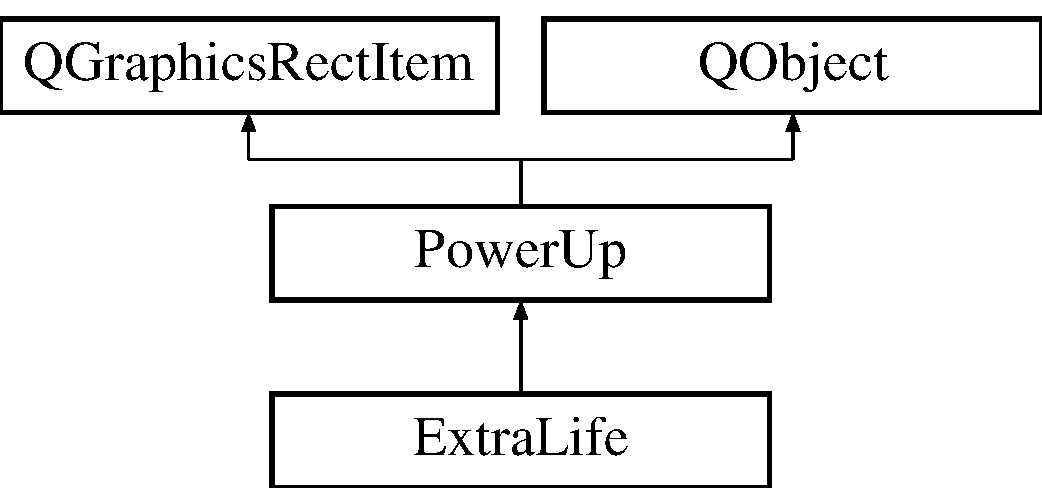
\includegraphics[height=3.000000cm]{class_extra_life}
\end{center}
\end{figure}
\subsection*{Public Member Functions}
\begin{DoxyCompactItemize}
\item 
\hypertarget{class_extra_life_a337b507790827e3d3179be14fef19737}{{\bfseries Extra\+Life} (const Q\+Rect\+F \&rect, Q\+String m\+\_\+title, qreal drop\+Velocity, const Q\+Brush \&fill\+\_\+brush=Q\+Brush())}\label{class_extra_life_a337b507790827e3d3179be14fef19737}

\item 
virtual void \hyperlink{class_extra_life_a2cfbfd8e3e7d33624a05c121ecc4ac82}{apply\+Bonus} ()
\begin{DoxyCompactList}\small\item\em Pure virtual class of the strategy design pattern. \end{DoxyCompactList}\end{DoxyCompactItemize}
\subsection*{Additional Inherited Members}


\subsection{Member Function Documentation}
\hypertarget{class_extra_life_a2cfbfd8e3e7d33624a05c121ecc4ac82}{\index{Extra\+Life@{Extra\+Life}!apply\+Bonus@{apply\+Bonus}}
\index{apply\+Bonus@{apply\+Bonus}!Extra\+Life@{Extra\+Life}}
\subsubsection[{apply\+Bonus}]{\setlength{\rightskip}{0pt plus 5cm}void Extra\+Life\+::apply\+Bonus (
\begin{DoxyParamCaption}
{}
\end{DoxyParamCaption}
)\hspace{0.3cm}{\ttfamily [virtual]}}}\label{class_extra_life_a2cfbfd8e3e7d33624a05c121ecc4ac82}


Pure virtual class of the strategy design pattern. 

\begin{DoxyReturn}{Returns}
void 
\end{DoxyReturn}


Implements \hyperlink{class_power_up}{Power\+Up}.



The documentation for this class was generated from the following files\+:\begin{DoxyCompactItemize}
\item 
/\+Users/khanh/\+I\+N\+F\+O3220\+\_\+\+Assignment/\+Assignment\+Three\+Base\+Two/extralife.\+h\item 
/\+Users/khanh/\+I\+N\+F\+O3220\+\_\+\+Assignment/\+Assignment\+Three\+Base\+Two/extralife.\+cpp\end{DoxyCompactItemize}

\hypertarget{class_level_generator}{\section{Level\+Generator Class Reference}
\label{class_level_generator}\index{Level\+Generator@{Level\+Generator}}
}
\subsection*{Public Member Functions}
\begin{DoxyCompactItemize}
\item 
\hyperlink{class_level_generator_abab5970ecff0044e9be203522a2d5f4a}{Level\+Generator} (int width, int height)
\begin{DoxyCompactList}\small\item\em Constructor for the \hyperlink{class_level_generator}{Level\+Generator} class. \end{DoxyCompactList}\item 
std\+::vector$<$ \hyperlink{class_brick}{Brick} $\ast$ $>$ \hyperlink{class_level_generator_ac4e73aa08a2267b9eff3d5c3ba25640b}{generate} (int level)
\begin{DoxyCompactList}\small\item\em Generates a new level of bricks based on the current level given. \end{DoxyCompactList}\end{DoxyCompactItemize}


\subsection{Constructor \& Destructor Documentation}
\hypertarget{class_level_generator_abab5970ecff0044e9be203522a2d5f4a}{\index{Level\+Generator@{Level\+Generator}!Level\+Generator@{Level\+Generator}}
\index{Level\+Generator@{Level\+Generator}!Level\+Generator@{Level\+Generator}}
\subsubsection[{Level\+Generator}]{\setlength{\rightskip}{0pt plus 5cm}Level\+Generator\+::\+Level\+Generator (
\begin{DoxyParamCaption}
\item[{int}]{width, }
\item[{int}]{height}
\end{DoxyParamCaption}
)}}\label{class_level_generator_abab5970ecff0044e9be203522a2d5f4a}


Constructor for the \hyperlink{class_level_generator}{Level\+Generator} class. 

\begin{DoxyReturn}{Returns}
\hyperlink{class_level_generator}{Level\+Generator} 
\end{DoxyReturn}


\subsection{Member Function Documentation}
\hypertarget{class_level_generator_ac4e73aa08a2267b9eff3d5c3ba25640b}{\index{Level\+Generator@{Level\+Generator}!generate@{generate}}
\index{generate@{generate}!Level\+Generator@{Level\+Generator}}
\subsubsection[{generate}]{\setlength{\rightskip}{0pt plus 5cm}std\+::vector$<$ {\bf Brick} $\ast$ $>$ Level\+Generator\+::generate (
\begin{DoxyParamCaption}
\item[{int}]{level}
\end{DoxyParamCaption}
)}}\label{class_level_generator_ac4e73aa08a2267b9eff3d5c3ba25640b}


Generates a new level of bricks based on the current level given. 


\begin{DoxyParams}{Parameters}
{\em int} & current level \\
\hline
\end{DoxyParams}
\begin{DoxyReturn}{Returns}
vector$<$\+Brick $\ast$$>$ which is a list of bricks 
\end{DoxyReturn}


The documentation for this class was generated from the following files\+:\begin{DoxyCompactItemize}
\item 
/\+Users/khanh/\+I\+N\+F\+O3220\+\_\+\+Assignment/\+Assignment\+Three\+Base\+Two/levelgenerator.\+h\item 
/\+Users/khanh/\+I\+N\+F\+O3220\+\_\+\+Assignment/\+Assignment\+Three\+Base\+Two/levelgenerator.\+cpp\end{DoxyCompactItemize}

\hypertarget{class_overlay_object}{\section{Overlay\+Object Class Reference}
\label{class_overlay_object}\index{Overlay\+Object@{Overlay\+Object}}
}
Inheritance diagram for Overlay\+Object\+:\begin{figure}[H]
\begin{center}
\leavevmode
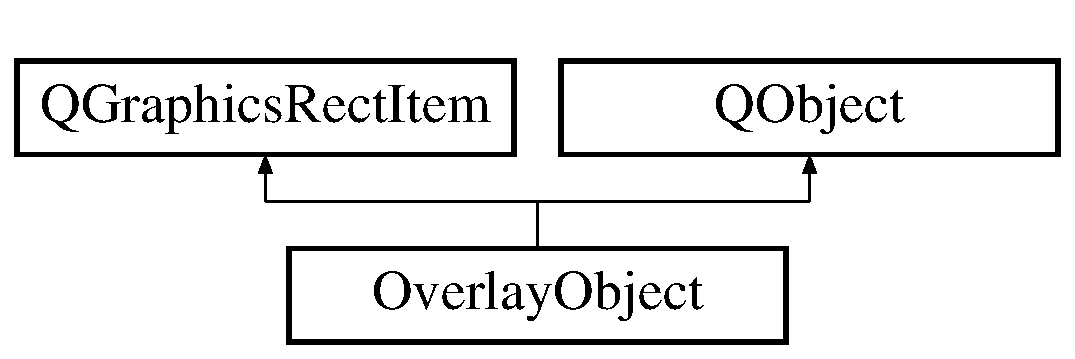
\includegraphics[height=2.000000cm]{class_overlay_object}
\end{center}
\end{figure}
\subsection*{Public Member Functions}
\begin{DoxyCompactItemize}
\item 
\hyperlink{class_overlay_object_a36e5d66953077671bce1086531f287c2}{Overlay\+Object} (const Q\+Rect\+F \&rect, bool visible, Q\+String title, Q\+String text)
\begin{DoxyCompactList}\small\item\em Constructor for the \hyperlink{class_overlay_object}{Overlay\+Object} class. \end{DoxyCompactList}\item 
void \hyperlink{class_overlay_object_ab7a69b842c942d9c5e24d44fbc5d150d}{set\+Text} (Q\+String new\+Text)
\begin{DoxyCompactList}\small\item\em Setter for the text. \end{DoxyCompactList}\item 
void \hyperlink{class_overlay_object_ad92a1142945e2bc7344ad4048d8916c8}{restore\+Default\+Text} ()
\begin{DoxyCompactList}\small\item\em Restores to the default text. \end{DoxyCompactList}\end{DoxyCompactItemize}
\subsection*{Protected Member Functions}
\begin{DoxyCompactItemize}
\item 
virtual void \hyperlink{class_overlay_object_a205f669215ddffd350a231421c77d33b}{advance} (int step)
\begin{DoxyCompactList}\small\item\em Handles the animation of the scene object. \end{DoxyCompactList}\item 
virtual void \hyperlink{class_overlay_object_ad028086b5c69cbb52d0bb5424c38d87d}{paint} (Q\+Painter $\ast$painter, const Q\+Style\+Option\+Graphics\+Item $\ast$option, Q\+Widget $\ast$widget)
\begin{DoxyCompactList}\small\item\em Draws the \hyperlink{class_overlay_object}{Overlay\+Object} onto the scene. \end{DoxyCompactList}\end{DoxyCompactItemize}


\subsection{Constructor \& Destructor Documentation}
\hypertarget{class_overlay_object_a36e5d66953077671bce1086531f287c2}{\index{Overlay\+Object@{Overlay\+Object}!Overlay\+Object@{Overlay\+Object}}
\index{Overlay\+Object@{Overlay\+Object}!Overlay\+Object@{Overlay\+Object}}
\subsubsection[{Overlay\+Object}]{\setlength{\rightskip}{0pt plus 5cm}Overlay\+Object\+::\+Overlay\+Object (
\begin{DoxyParamCaption}
\item[{const Q\+Rect\+F \&}]{rect, }
\item[{bool}]{visible, }
\item[{Q\+String}]{title, }
\item[{Q\+String}]{text}
\end{DoxyParamCaption}
)}}\label{class_overlay_object_a36e5d66953077671bce1086531f287c2}


Constructor for the \hyperlink{class_overlay_object}{Overlay\+Object} class. 


\begin{DoxyParams}{Parameters}
{\em Q\+Rect\+F} & \&rect which is the rectangle (coordinate and size) \\
\hline
{\em bool} & visible which determines if the overlay will be visible on the scene or not \\
\hline
{\em Q\+String} & title which identifies the overlay \\
\hline
{\em Q\+String} & text which is the text displayed on the scene \\
\hline
\end{DoxyParams}
\begin{DoxyReturn}{Returns}
\hyperlink{class_overlay_object}{Overlay\+Object} 
\end{DoxyReturn}


\subsection{Member Function Documentation}
\hypertarget{class_overlay_object_a205f669215ddffd350a231421c77d33b}{\index{Overlay\+Object@{Overlay\+Object}!advance@{advance}}
\index{advance@{advance}!Overlay\+Object@{Overlay\+Object}}
\subsubsection[{advance}]{\setlength{\rightskip}{0pt plus 5cm}void Overlay\+Object\+::advance (
\begin{DoxyParamCaption}
\item[{int}]{step}
\end{DoxyParamCaption}
)\hspace{0.3cm}{\ttfamily [protected]}, {\ttfamily [virtual]}}}\label{class_overlay_object_a205f669215ddffd350a231421c77d33b}


Handles the animation of the scene object. 

\begin{DoxyReturn}{Returns}
void 
\end{DoxyReturn}
\hypertarget{class_overlay_object_ad028086b5c69cbb52d0bb5424c38d87d}{\index{Overlay\+Object@{Overlay\+Object}!paint@{paint}}
\index{paint@{paint}!Overlay\+Object@{Overlay\+Object}}
\subsubsection[{paint}]{\setlength{\rightskip}{0pt plus 5cm}void Overlay\+Object\+::paint (
\begin{DoxyParamCaption}
\item[{Q\+Painter $\ast$}]{painter, }
\item[{const Q\+Style\+Option\+Graphics\+Item $\ast$}]{option, }
\item[{Q\+Widget $\ast$}]{widget}
\end{DoxyParamCaption}
)\hspace{0.3cm}{\ttfamily [protected]}, {\ttfamily [virtual]}}}\label{class_overlay_object_ad028086b5c69cbb52d0bb5424c38d87d}


Draws the \hyperlink{class_overlay_object}{Overlay\+Object} onto the scene. 

\begin{DoxyReturn}{Returns}
void 
\end{DoxyReturn}
\hypertarget{class_overlay_object_ad92a1142945e2bc7344ad4048d8916c8}{\index{Overlay\+Object@{Overlay\+Object}!restore\+Default\+Text@{restore\+Default\+Text}}
\index{restore\+Default\+Text@{restore\+Default\+Text}!Overlay\+Object@{Overlay\+Object}}
\subsubsection[{restore\+Default\+Text}]{\setlength{\rightskip}{0pt plus 5cm}void Overlay\+Object\+::restore\+Default\+Text (
\begin{DoxyParamCaption}
{}
\end{DoxyParamCaption}
)}}\label{class_overlay_object_ad92a1142945e2bc7344ad4048d8916c8}


Restores to the default text. 

\begin{DoxyReturn}{Returns}
void 
\end{DoxyReturn}
\hypertarget{class_overlay_object_ab7a69b842c942d9c5e24d44fbc5d150d}{\index{Overlay\+Object@{Overlay\+Object}!set\+Text@{set\+Text}}
\index{set\+Text@{set\+Text}!Overlay\+Object@{Overlay\+Object}}
\subsubsection[{set\+Text}]{\setlength{\rightskip}{0pt plus 5cm}void Overlay\+Object\+::set\+Text (
\begin{DoxyParamCaption}
\item[{Q\+String}]{new\+Text}
\end{DoxyParamCaption}
)}}\label{class_overlay_object_ab7a69b842c942d9c5e24d44fbc5d150d}


Setter for the text. 


\begin{DoxyParams}{Parameters}
{\em Q\+String} & new\+Text which is the text that the \hyperlink{class_overlay_object}{Overlay\+Object} take on. \\
\hline
\end{DoxyParams}
\begin{DoxyReturn}{Returns}
void 
\end{DoxyReturn}


The documentation for this class was generated from the following files\+:\begin{DoxyCompactItemize}
\item 
/\+Users/khanh/\+I\+N\+F\+O3220\+\_\+\+Assignment/\+Assignment\+Three\+Base\+Two/overlayobject.\+h\item 
/\+Users/khanh/\+I\+N\+F\+O3220\+\_\+\+Assignment/\+Assignment\+Three\+Base\+Two/overlayobject.\+cpp\end{DoxyCompactItemize}

\hypertarget{class_paddle}{\section{Paddle Class Reference}
\label{class_paddle}\index{Paddle@{Paddle}}
}
Inheritance diagram for Paddle\+:\begin{figure}[H]
\begin{center}
\leavevmode
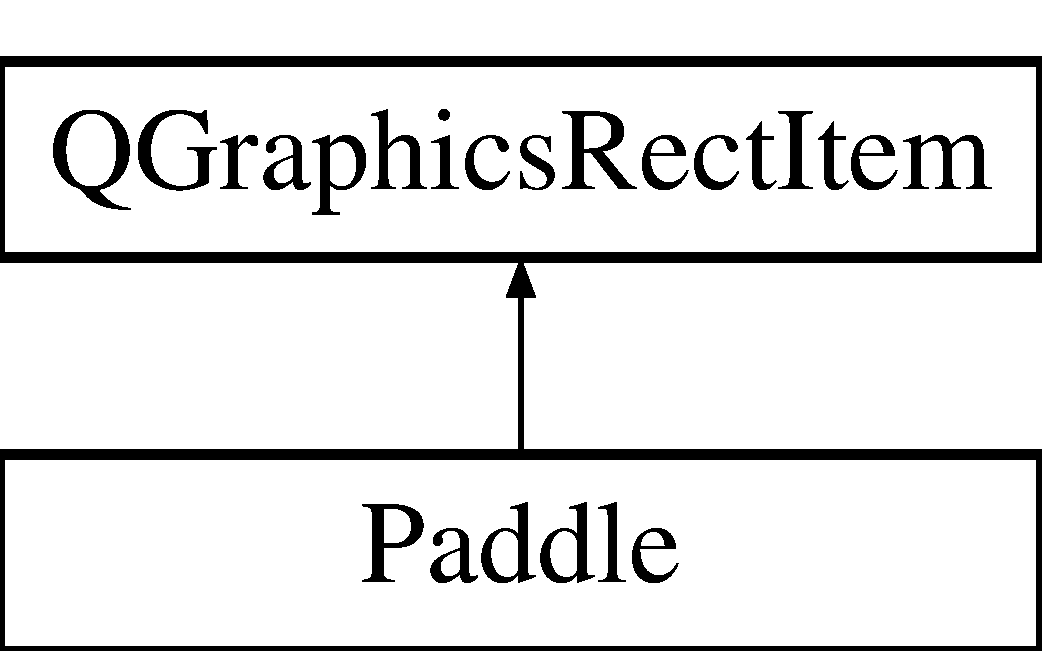
\includegraphics[height=2.000000cm]{class_paddle}
\end{center}
\end{figure}
\subsection*{Public Member Functions}
\begin{DoxyCompactItemize}
\item 
\hypertarget{class_paddle_a9e39beea49fb243ff115fd5eb79fed48}{{\bfseries Paddle} (const Q\+Rect\+F \&rect, const Q\+Brush \&fill\+\_\+brush=Q\+Brush())}\label{class_paddle_a9e39beea49fb243ff115fd5eb79fed48}

\end{DoxyCompactItemize}
\subsection*{Protected Member Functions}
\begin{DoxyCompactItemize}
\item 
virtual void \hyperlink{class_paddle_a77583765e1527e433e9c13fb38c947cf}{advance} (int step)
\begin{DoxyCompactList}\small\item\em Sets the state of the brick as the frame of the scene is advancing. \end{DoxyCompactList}\item 
virtual void \hyperlink{class_paddle_a7b53c543e3fa8d4118a19a0b0ba3f07f}{paint} (Q\+Painter $\ast$painter, const Q\+Style\+Option\+Graphics\+Item $\ast$option, Q\+Widget $\ast$widget)
\begin{DoxyCompactList}\small\item\em Paints the paddle object. \end{DoxyCompactList}\end{DoxyCompactItemize}


\subsection{Member Function Documentation}
\hypertarget{class_paddle_a77583765e1527e433e9c13fb38c947cf}{\index{Paddle@{Paddle}!advance@{advance}}
\index{advance@{advance}!Paddle@{Paddle}}
\subsubsection[{advance}]{\setlength{\rightskip}{0pt plus 5cm}void Paddle\+::advance (
\begin{DoxyParamCaption}
\item[{int}]{step}
\end{DoxyParamCaption}
)\hspace{0.3cm}{\ttfamily [protected]}, {\ttfamily [virtual]}}}\label{class_paddle_a77583765e1527e433e9c13fb38c947cf}


Sets the state of the brick as the frame of the scene is advancing. 

Called by the advance method of the parent Table.

This method is called twice. The first time with step == 0 to indicate the scene is about to advance, and a second time with step == 1 to indicate the scene is advancing.


\begin{DoxyParams}{Parameters}
{\em step} & \\
\hline
\end{DoxyParams}
\hypertarget{class_paddle_a7b53c543e3fa8d4118a19a0b0ba3f07f}{\index{Paddle@{Paddle}!paint@{paint}}
\index{paint@{paint}!Paddle@{Paddle}}
\subsubsection[{paint}]{\setlength{\rightskip}{0pt plus 5cm}void Paddle\+::paint (
\begin{DoxyParamCaption}
\item[{Q\+Painter $\ast$}]{painter, }
\item[{const Q\+Style\+Option\+Graphics\+Item $\ast$}]{option, }
\item[{Q\+Widget $\ast$}]{widget}
\end{DoxyParamCaption}
)\hspace{0.3cm}{\ttfamily [protected]}, {\ttfamily [virtual]}}}\label{class_paddle_a7b53c543e3fa8d4118a19a0b0ba3f07f}


Paints the paddle object. 

Performs the painting of the brick in the parent Table object using the given painter.


\begin{DoxyParams}{Parameters}
{\em painter} & in which to perform painting \\
\hline
\end{DoxyParams}


The documentation for this class was generated from the following files\+:\begin{DoxyCompactItemize}
\item 
/\+Users/khanh/\+I\+N\+F\+O3220\+\_\+\+Assignment/\+Assignment\+Three\+Base\+Two/paddle.\+h\item 
/\+Users/khanh/\+I\+N\+F\+O3220\+\_\+\+Assignment/\+Assignment\+Three\+Base\+Two/paddle.\+cpp\end{DoxyCompactItemize}

\hypertarget{class_player}{\section{Player Class Reference}
\label{class_player}\index{Player@{Player}}
}
\subsection*{Public Member Functions}
\begin{DoxyCompactItemize}
\item 
\hypertarget{class_player_a338911228050aac83209fc91f459ad6a}{{\bfseries Player} (int lives, bool level\+Gen, bool power\+Ups)}\label{class_player_a338911228050aac83209fc91f459ad6a}

\item 
\hypertarget{class_player_af56ac33b9b2ebd9f97c8a6f485cf2d47}{int {\bfseries get\+Lives} ()}\label{class_player_af56ac33b9b2ebd9f97c8a6f485cf2d47}

\item 
\hypertarget{class_player_a97e5447778ae6c384eedc532dcd8431d}{int {\bfseries get\+Score} ()}\label{class_player_a97e5447778ae6c384eedc532dcd8431d}

\item 
\hypertarget{class_player_a3c1737f7d71990bf2c6a7d655e4e7477}{int {\bfseries get\+Current\+Level} ()}\label{class_player_a3c1737f7d71990bf2c6a7d655e4e7477}

\item 
\hypertarget{class_player_acea3402d95e62499acd9cf4a37cb3a96}{bool {\bfseries get\+Round\+Started} ()}\label{class_player_acea3402d95e62499acd9cf4a37cb3a96}

\item 
\hypertarget{class_player_a830e302da448a75b8ecd8def6608ff30}{int {\bfseries increment\+Life} ()}\label{class_player_a830e302da448a75b8ecd8def6608ff30}

\item 
\hypertarget{class_player_a62ca25abc6407794000523c1f7bda649}{int {\bfseries decrement\+Life} ()}\label{class_player_a62ca25abc6407794000523c1f7bda649}

\item 
\hypertarget{class_player_a4ffc60110201dcbedc0c83e7b067bed9}{int {\bfseries increase\+Score} (int val)}\label{class_player_a4ffc60110201dcbedc0c83e7b067bed9}

\item 
\hypertarget{class_player_acd7d911c585110e7a05c5c270a5ab35a}{int {\bfseries increase\+Current\+Level} ()}\label{class_player_acd7d911c585110e7a05c5c270a5ab35a}

\item 
\hypertarget{class_player_ac90d16287b2569050c652d4fb20424ed}{bool {\bfseries set\+Round\+Started} (bool val)}\label{class_player_ac90d16287b2569050c652d4fb20424ed}

\item 
\hypertarget{class_player_a9e5dc273ee10345d49be88f07a19d0aa}{bool {\bfseries get\+Level\+Gen} ()}\label{class_player_a9e5dc273ee10345d49be88f07a19d0aa}

\item 
\hypertarget{class_player_a061abc3a6fd39a93add484f4a57ad6d5}{bool {\bfseries get\+Power\+Ups} ()}\label{class_player_a061abc3a6fd39a93add484f4a57ad6d5}

\item 
\hypertarget{class_player_ad85b7618b95a6d763db0587760fd2dd3}{void {\bfseries reset\+Stats} ()}\label{class_player_ad85b7618b95a6d763db0587760fd2dd3}

\end{DoxyCompactItemize}


The documentation for this class was generated from the following files\+:\begin{DoxyCompactItemize}
\item 
/\+Users/khanh/\+I\+N\+F\+O3220\+\_\+\+Assignment/\+Assignment\+Three\+Base\+Two/player.\+h\item 
/\+Users/khanh/\+I\+N\+F\+O3220\+\_\+\+Assignment/\+Assignment\+Three\+Base\+Two/player.\+cpp\end{DoxyCompactItemize}

\hypertarget{class_power_up}{\section{Power\+Up Class Reference}
\label{class_power_up}\index{Power\+Up@{Power\+Up}}
}
Inheritance diagram for Power\+Up\+:\begin{figure}[H]
\begin{center}
\leavevmode
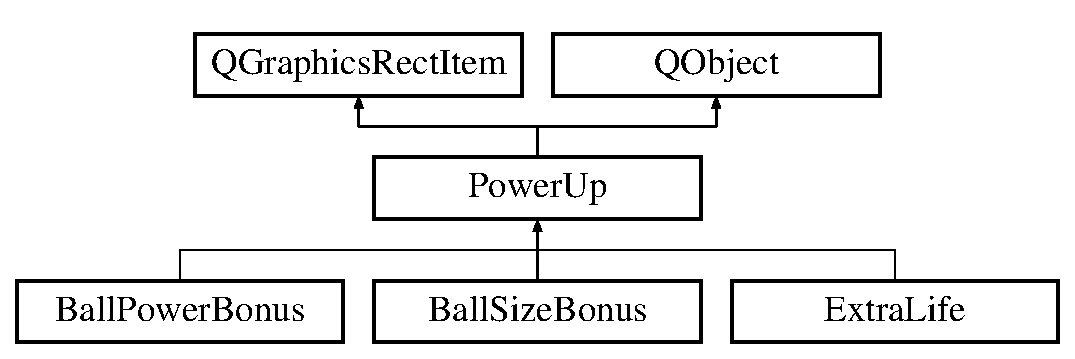
\includegraphics[height=3.000000cm]{class_power_up}
\end{center}
\end{figure}
\subsection*{Public Member Functions}
\begin{DoxyCompactItemize}
\item 
\hyperlink{class_power_up_a0358fe89144d73b501e2720abf633481}{Power\+Up} (const Q\+Rect\+F \&rect, Q\+String m\+\_\+title, qreal drop\+Velocity, const Q\+Brush \&fill\+\_\+brush=Q\+Brush())
\begin{DoxyCompactList}\small\item\em Constructor of the \hyperlink{class_power_up}{Power\+Up} class. \end{DoxyCompactList}\item 
\hypertarget{class_power_up_aab9ea5afffada47bb0f20d8d69e41843}{virtual void {\bfseries apply\+Bonus} ()=0}\label{class_power_up_aab9ea5afffada47bb0f20d8d69e41843}

\end{DoxyCompactItemize}
\subsection*{Protected Member Functions}
\begin{DoxyCompactItemize}
\item 
virtual void \hyperlink{class_power_up_af24a16c7eba69136b408540cb0866a9b}{advance} (int step)
\begin{DoxyCompactList}\small\item\em Sets the state of the powerup as the frame of the scene is advancing. \end{DoxyCompactList}\item 
virtual void \hyperlink{class_power_up_a12700945cf46c42f38a7e5f4f18a2595}{paint} (Q\+Painter $\ast$painter, const Q\+Style\+Option\+Graphics\+Item $\ast$option, Q\+Widget $\ast$widget)
\begin{DoxyCompactList}\small\item\em Paints the powerup object. \end{DoxyCompactList}\end{DoxyCompactItemize}


\subsection{Constructor \& Destructor Documentation}
\hypertarget{class_power_up_a0358fe89144d73b501e2720abf633481}{\index{Power\+Up@{Power\+Up}!Power\+Up@{Power\+Up}}
\index{Power\+Up@{Power\+Up}!Power\+Up@{Power\+Up}}
\subsubsection[{Power\+Up}]{\setlength{\rightskip}{0pt plus 5cm}Power\+Up\+::\+Power\+Up (
\begin{DoxyParamCaption}
\item[{const Q\+Rect\+F \&}]{rect, }
\item[{Q\+String}]{title, }
\item[{qreal}]{drop\+Velocity, }
\item[{const Q\+Brush \&}]{fill\+\_\+brush = {\ttfamily QBrush()}}
\end{DoxyParamCaption}
)}}\label{class_power_up_a0358fe89144d73b501e2720abf633481}


Constructor of the \hyperlink{class_power_up}{Power\+Up} class. 

\begin{DoxyReturn}{Returns}
void 
\end{DoxyReturn}


\subsection{Member Function Documentation}
\hypertarget{class_power_up_af24a16c7eba69136b408540cb0866a9b}{\index{Power\+Up@{Power\+Up}!advance@{advance}}
\index{advance@{advance}!Power\+Up@{Power\+Up}}
\subsubsection[{advance}]{\setlength{\rightskip}{0pt plus 5cm}void Power\+Up\+::advance (
\begin{DoxyParamCaption}
\item[{int}]{step}
\end{DoxyParamCaption}
)\hspace{0.3cm}{\ttfamily [protected]}, {\ttfamily [virtual]}}}\label{class_power_up_af24a16c7eba69136b408540cb0866a9b}


Sets the state of the powerup as the frame of the scene is advancing. 

Called by the advance method of the parent Table.

This method is called twice. The first time with step == 0 to indicate the scene is about to advance, and a second time with step == 1 to indicate the scene is advancing.


\begin{DoxyParams}{Parameters}
{\em step} & \\
\hline
\end{DoxyParams}
\hypertarget{class_power_up_a12700945cf46c42f38a7e5f4f18a2595}{\index{Power\+Up@{Power\+Up}!paint@{paint}}
\index{paint@{paint}!Power\+Up@{Power\+Up}}
\subsubsection[{paint}]{\setlength{\rightskip}{0pt plus 5cm}void Power\+Up\+::paint (
\begin{DoxyParamCaption}
\item[{Q\+Painter $\ast$}]{painter, }
\item[{const Q\+Style\+Option\+Graphics\+Item $\ast$}]{option, }
\item[{Q\+Widget $\ast$}]{widget}
\end{DoxyParamCaption}
)\hspace{0.3cm}{\ttfamily [protected]}, {\ttfamily [virtual]}}}\label{class_power_up_a12700945cf46c42f38a7e5f4f18a2595}


Paints the powerup object. 

Performs the painting of the powerup in the parent Table object using the given painter.


\begin{DoxyParams}{Parameters}
{\em painter} & in which to perform painting \\
\hline
\end{DoxyParams}


The documentation for this class was generated from the following files\+:\begin{DoxyCompactItemize}
\item 
/\+Users/khanh/\+I\+N\+F\+O3220\+\_\+\+Assignment/\+Assignment\+Three\+Base\+Two/powerup.\+h\item 
/\+Users/khanh/\+I\+N\+F\+O3220\+\_\+\+Assignment/\+Assignment\+Three\+Base\+Two/powerup.\+cpp\end{DoxyCompactItemize}

\hypertarget{class_table_scene}{\section{Table\+Scene Class Reference}
\label{class_table_scene}\index{Table\+Scene@{Table\+Scene}}
}
Inheritance diagram for Table\+Scene\+:\begin{figure}[H]
\begin{center}
\leavevmode
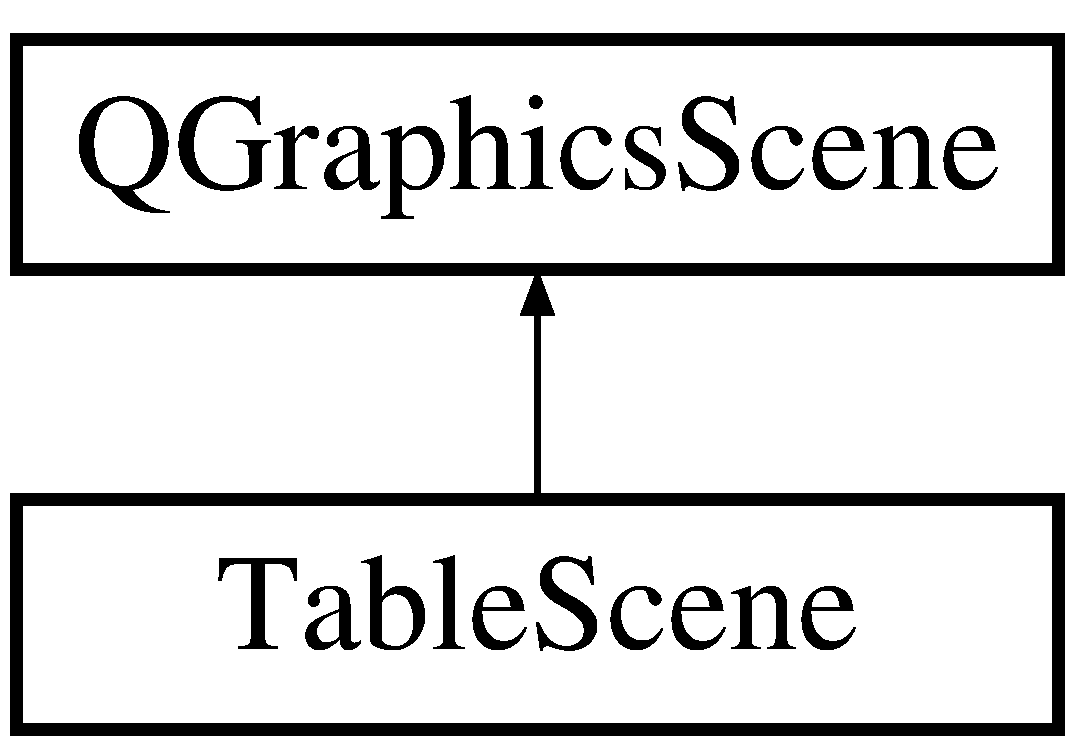
\includegraphics[height=2.000000cm]{class_table_scene}
\end{center}
\end{figure}
\subsection*{Public Member Functions}
\begin{DoxyCompactItemize}
\item 
void \hyperlink{class_table_scene_a89034a773135a994fe062b529bfaa644}{start\+Animation} (int framerate)
\begin{DoxyCompactList}\small\item\em Start the timer with the provided framerate. \end{DoxyCompactList}\item 
\hypertarget{class_table_scene_ad7a7f185444aaabac14bff225f439ae1}{Q\+Graphics\+View \& \hyperlink{class_table_scene_ad7a7f185444aaabac14bff225f439ae1}{view} ()}\label{class_table_scene_ad7a7f185444aaabac14bff225f439ae1}

\begin{DoxyCompactList}\small\item\em Getter for the \hyperlink{class_table_view}{Table\+View} of the table. \end{DoxyCompactList}\item 
\hyperlink{class_table_scene}{Table\+Scene} \& \hyperlink{class_table_scene_ae9f0ee4cdf943de16434a8095a44c1e5}{add\+Ball} (\hyperlink{class_ball}{Ball} $\ast$ball)
\begin{DoxyCompactList}\small\item\em Adds the ball to the scene. \end{DoxyCompactList}\item 
\hypertarget{class_table_scene_ae78eb6707dc5f8e6dff5989015e08e6f}{\hyperlink{class_ball}{Ball} $\ast$ \hyperlink{class_table_scene_ae78eb6707dc5f8e6dff5989015e08e6f}{get\+Ball} ()}\label{class_table_scene_ae78eb6707dc5f8e6dff5989015e08e6f}

\begin{DoxyCompactList}\small\item\em Getter for ball. \end{DoxyCompactList}\item 
\hyperlink{class_table_scene}{Table\+Scene} \& \hyperlink{class_table_scene_a617500b63b8d660a6f4f2807bb78a3e5}{add\+Brick} (\hyperlink{class_brick}{Brick} $\ast$brick)
\begin{DoxyCompactList}\small\item\em Adds the brick to the scene. \end{DoxyCompactList}\item 
std\+::vector$<$ \hyperlink{class_brick}{Brick} $\ast$ $>$ \& \hyperlink{class_table_scene_ab49b9da80894742da850699e9d09ae50}{get\+Bricks} ()
\begin{DoxyCompactList}\small\item\em Gets the vector of \hyperlink{class_brick}{Brick} pointers. \end{DoxyCompactList}\item 
\hyperlink{class_table_scene}{Table\+Scene} \& \hyperlink{class_table_scene_afea73d45fab7221c91177d9b7b385b63}{remove\+Brick} (\hyperlink{class_brick}{Brick} $\ast$brick)
\begin{DoxyCompactList}\small\item\em Removes the brick from the scene. \end{DoxyCompactList}\item 
\hypertarget{class_table_scene_abacaa9ebff0060101dfd63c948c661af}{\hyperlink{class_table_scene}{Table\+Scene} \& \hyperlink{class_table_scene_abacaa9ebff0060101dfd63c948c661af}{add\+Paddle} (\hyperlink{class_paddle}{Paddle} $\ast$paddle)}\label{class_table_scene_abacaa9ebff0060101dfd63c948c661af}

\begin{DoxyCompactList}\small\item\em Adder for \hyperlink{class_paddle}{Paddle} objects. \end{DoxyCompactList}\item 
\hypertarget{class_table_scene_a889ae59e16d18200d13ec81d47b3aba5}{\hyperlink{class_paddle}{Paddle} $\ast$ \hyperlink{class_table_scene_a889ae59e16d18200d13ec81d47b3aba5}{get\+Paddle} ()}\label{class_table_scene_a889ae59e16d18200d13ec81d47b3aba5}

\begin{DoxyCompactList}\small\item\em Getter for ball. \end{DoxyCompactList}\item 
\hypertarget{class_table_scene_aefde46bcdf0513f10b1d3dc62b60cbc9}{\hyperlink{class_table_scene}{Table\+Scene} \& \hyperlink{class_table_scene_aefde46bcdf0513f10b1d3dc62b60cbc9}{add\+Overlay\+Object} (\hyperlink{class_overlay_object}{Overlay\+Object} $\ast$overlay)}\label{class_table_scene_aefde46bcdf0513f10b1d3dc62b60cbc9}

\begin{DoxyCompactList}\small\item\em adder for Overlay\+Objects \end{DoxyCompactList}\item 
\hypertarget{class_table_scene_ae92209b5c74ae7f4ba6d3872aa2578db}{std\+::vector$<$ \hyperlink{class_overlay_object}{Overlay\+Object} $\ast$ $>$ \& \hyperlink{class_table_scene_ae92209b5c74ae7f4ba6d3872aa2578db}{get\+Overlay\+Objects} ()}\label{class_table_scene_ae92209b5c74ae7f4ba6d3872aa2578db}

\begin{DoxyCompactList}\small\item\em getter for Overlay\+Objects \end{DoxyCompactList}\item 
\hypertarget{class_table_scene_adc85426c14e38ddc222ff62a7f25743f}{void \hyperlink{class_table_scene_adc85426c14e38ddc222ff62a7f25743f}{update\+Overlay} (int index, Q\+String)}\label{class_table_scene_adc85426c14e38ddc222ff62a7f25743f}

\begin{DoxyCompactList}\small\item\em mutator for overlays \end{DoxyCompactList}\item 
\hypertarget{class_table_scene_abda1811e505edc8058155c01795e6740}{bool \hyperlink{class_table_scene_abda1811e505edc8058155c01795e6740}{get\+Play\+Game} ()}\label{class_table_scene_abda1811e505edc8058155c01795e6740}

\begin{DoxyCompactList}\small\item\em Getter for the play\+Game bool. \end{DoxyCompactList}\item 
\hypertarget{class_table_scene_a4fb355f5bd6ea8973e82404bf8cc1bc9}{void \hyperlink{class_table_scene_a4fb355f5bd6ea8973e82404bf8cc1bc9}{set\+Player} (\hyperlink{class_player}{Player} $\ast$player)}\label{class_table_scene_a4fb355f5bd6ea8973e82404bf8cc1bc9}

\begin{DoxyCompactList}\small\item\em Setter for player member variable. \end{DoxyCompactList}\item 
\hypertarget{class_table_scene_a33af3ee1dc5da4402df15578a59cc33a}{\hyperlink{class_player}{Player} $\ast$ \hyperlink{class_table_scene_a33af3ee1dc5da4402df15578a59cc33a}{get\+Player} ()}\label{class_table_scene_a33af3ee1dc5da4402df15578a59cc33a}

\begin{DoxyCompactList}\small\item\em Getter for the player. \end{DoxyCompactList}\item 
\hypertarget{class_table_scene_abae467079a839a7adf5eeced33189253}{void \hyperlink{class_table_scene_abae467079a839a7adf5eeced33189253}{generate\+Level} ()}\label{class_table_scene_abae467079a839a7adf5eeced33189253}

\begin{DoxyCompactList}\small\item\em Generate next level using the \hyperlink{class_level_generator}{Level\+Generator}. \end{DoxyCompactList}\item 
void \hyperlink{class_table_scene_aa84f2a633bab238f7883954f05a9ec74}{restart\+Game} ()
\begin{DoxyCompactList}\small\item\em Restarts the game. \end{DoxyCompactList}\item 
\hypertarget{class_table_scene_a3f42c598fe7e8f18271a34582a9daea8}{void \hyperlink{class_table_scene_a3f42c598fe7e8f18271a34582a9daea8}{add\+Powerup} (qreal x, qreal y)}\label{class_table_scene_a3f42c598fe7e8f18271a34582a9daea8}

\begin{DoxyCompactList}\small\item\em Chance for a \hyperlink{class_power_up}{Power\+Up} to drop after a brick has died. \end{DoxyCompactList}\item 
\hypertarget{class_table_scene_abe0a8dfbb359ae6363af75c093f17f99}{void \hyperlink{class_table_scene_abe0a8dfbb359ae6363af75c093f17f99}{reset\+Power\+Ups} ()}\label{class_table_scene_abe0a8dfbb359ae6363af75c093f17f99}

\begin{DoxyCompactList}\small\item\em Resets \hyperlink{class_power_up}{Power\+Up} bonuses. \end{DoxyCompactList}\item 
\hypertarget{class_table_scene_a28aeeac53bdc7570630d62b7872b1b37}{virtual \hyperlink{class_table_scene_a28aeeac53bdc7570630d62b7872b1b37}{$\sim$\+Table\+Scene} ()}\label{class_table_scene_a28aeeac53bdc7570630d62b7872b1b37}

\begin{DoxyCompactList}\small\item\em \hyperlink{class_table_scene}{Table\+Scene} destructor. \end{DoxyCompactList}\end{DoxyCompactItemize}
\subsection*{Static Public Member Functions}
\begin{DoxyCompactItemize}
\item 
static \hyperlink{class_table_scene}{Table\+Scene} $\ast$ \hyperlink{class_table_scene_a9c9586a5d3a44e6924724b08af889cc5}{instance} (int width, int height, Q\+Color bg\+Colour, bool play\+Game)
\begin{DoxyCompactList}\small\item\em Getter for the single table instance. \end{DoxyCompactList}\end{DoxyCompactItemize}
\subsection*{Protected Member Functions}
\begin{DoxyCompactItemize}
\item 
\hyperlink{class_table_scene_aa130b4504c41933d28f83d707250592f}{Table\+Scene} (int width, int height, Q\+Color bg\+Colour, bool play\+Game)
\begin{DoxyCompactList}\small\item\em \hyperlink{class_table_scene}{Table\+Scene} constructor. \end{DoxyCompactList}\item 
\hypertarget{class_table_scene_aa0cf9de7b0d0b277f22fa743169d5679}{void \hyperlink{class_table_scene_aa0cf9de7b0d0b277f22fa743169d5679}{stop\+Animation} ()}\label{class_table_scene_aa0cf9de7b0d0b277f22fa743169d5679}

\begin{DoxyCompactList}\small\item\em Stop the timer. \end{DoxyCompactList}\item 
\hypertarget{class_table_scene_aa4cf493a3e1764d7a71a3cca8e02e476}{void \hyperlink{class_table_scene_aa4cf493a3e1764d7a71a3cca8e02e476}{restart\+Animation} ()}\label{class_table_scene_aa4cf493a3e1764d7a71a3cca8e02e476}

\begin{DoxyCompactList}\small\item\em Restart the timer. \end{DoxyCompactList}\item 
\hypertarget{class_table_scene_a8af53c9bb4da1dbadaa337c60473b24d}{void \hyperlink{class_table_scene_a8af53c9bb4da1dbadaa337c60473b24d}{toggle\+Animation} ()}\label{class_table_scene_a8af53c9bb4da1dbadaa337c60473b24d}

\begin{DoxyCompactList}\small\item\em Toggles the timer. \end{DoxyCompactList}\item 
virtual void \hyperlink{class_table_scene_adf3ccbff20b72a0badc1cb0d3f4e9e67}{key\+Press\+Event} (Q\+Key\+Event $\ast$event)
\begin{DoxyCompactList}\small\item\em Overidden key\+Press\+Event to handle animation toggle. \end{DoxyCompactList}\item 
virtual void \hyperlink{class_table_scene_a90f09546716546a0132e89cde6fa6407}{mouse\+Move\+Event} (Q\+Graphics\+Scene\+Mouse\+Event $\ast$event)
\begin{DoxyCompactList}\small\item\em Handles mouse movement events. This method controls the paddle's movement. \end{DoxyCompactList}\item 
virtual void \hyperlink{class_table_scene_adff7918b7b6041d6ec4f30542686c5d0}{mouse\+Press\+Event} (Q\+Graphics\+Scene\+Mouse\+Event $\ast$event)
\begin{DoxyCompactList}\small\item\em Handles mouse press events. This method controls the launching of the ball. \end{DoxyCompactList}\end{DoxyCompactItemize}


\subsection{Constructor \& Destructor Documentation}
\hypertarget{class_table_scene_aa130b4504c41933d28f83d707250592f}{\index{Table\+Scene@{Table\+Scene}!Table\+Scene@{Table\+Scene}}
\index{Table\+Scene@{Table\+Scene}!Table\+Scene@{Table\+Scene}}
\subsubsection[{Table\+Scene}]{\setlength{\rightskip}{0pt plus 5cm}Table\+Scene\+::\+Table\+Scene (
\begin{DoxyParamCaption}
\item[{int}]{width, }
\item[{int}]{height, }
\item[{Q\+Color}]{bg\+Colour, }
\item[{bool}]{play\+Game}
\end{DoxyParamCaption}
)\hspace{0.3cm}{\ttfamily [protected]}}}\label{class_table_scene_aa130b4504c41933d28f83d707250592f}


\hyperlink{class_table_scene}{Table\+Scene} constructor. 


\begin{DoxyParams}{Parameters}
{\em width} & width of table \\
\hline
{\em height} & height of table \\
\hline
{\em bg\+Colour} & Q\+Color background colour of table \\
\hline
{\em min\+Width} & minimum width of the table (if resizable) \\
\hline
{\em min\+Height} & minimum height of the table (if resizable) \\
\hline
{\em max\+Width} & maximum width of the table (if resizable) \\
\hline
{\em max\+Height} & maximum height of the table (if resizable) \\
\hline
{\em resizable} & indicates whether the table window is resizable \\
\hline
\end{DoxyParams}


\subsection{Member Function Documentation}
\hypertarget{class_table_scene_ae9f0ee4cdf943de16434a8095a44c1e5}{\index{Table\+Scene@{Table\+Scene}!add\+Ball@{add\+Ball}}
\index{add\+Ball@{add\+Ball}!Table\+Scene@{Table\+Scene}}
\subsubsection[{add\+Ball}]{\setlength{\rightskip}{0pt plus 5cm}{\bf Table\+Scene} \& Table\+Scene\+::add\+Ball (
\begin{DoxyParamCaption}
\item[{{\bf Ball} $\ast$}]{ball}
\end{DoxyParamCaption}
)}}\label{class_table_scene_ae9f0ee4cdf943de16434a8095a44c1e5}


Adds the ball to the scene. 

A wrapper for add\+Item that additionally keeps track of the ball pointer for easy reference.

Transfers ownership of the ball to the table.


\begin{DoxyParams}{Parameters}
{\em \hyperlink{class_ball}{Ball}} & pointer to the ball \\
\hline
\end{DoxyParams}
\hypertarget{class_table_scene_a617500b63b8d660a6f4f2807bb78a3e5}{\index{Table\+Scene@{Table\+Scene}!add\+Brick@{add\+Brick}}
\index{add\+Brick@{add\+Brick}!Table\+Scene@{Table\+Scene}}
\subsubsection[{add\+Brick}]{\setlength{\rightskip}{0pt plus 5cm}{\bf Table\+Scene} \& Table\+Scene\+::add\+Brick (
\begin{DoxyParamCaption}
\item[{{\bf Brick} $\ast$}]{brick}
\end{DoxyParamCaption}
)}}\label{class_table_scene_a617500b63b8d660a6f4f2807bb78a3e5}


Adds the brick to the scene. 

A wrapper for add\+Item that additionally keeps track of the brick pointers for easy reference.

Transfers ownership of the brick to the table.

Bricks that overlap with existing objects are abandoned


\begin{DoxyParams}{Parameters}
{\em \hyperlink{class_brick}{Brick}} & pointer to the brick \\
\hline
\end{DoxyParams}
\hypertarget{class_table_scene_ab49b9da80894742da850699e9d09ae50}{\index{Table\+Scene@{Table\+Scene}!get\+Bricks@{get\+Bricks}}
\index{get\+Bricks@{get\+Bricks}!Table\+Scene@{Table\+Scene}}
\subsubsection[{get\+Bricks}]{\setlength{\rightskip}{0pt plus 5cm}std\+::vector$<$ {\bf Brick} $\ast$ $>$ \& Table\+Scene\+::get\+Bricks (
\begin{DoxyParamCaption}
{}
\end{DoxyParamCaption}
)}}\label{class_table_scene_ab49b9da80894742da850699e9d09ae50}


Gets the vector of \hyperlink{class_brick}{Brick} pointers. 

\begin{DoxyReturn}{Returns}
\hyperlink{class_table_scene}{Table\+Scene} for chaining 
\end{DoxyReturn}
\hypertarget{class_table_scene_a9c9586a5d3a44e6924724b08af889cc5}{\index{Table\+Scene@{Table\+Scene}!instance@{instance}}
\index{instance@{instance}!Table\+Scene@{Table\+Scene}}
\subsubsection[{instance}]{\setlength{\rightskip}{0pt plus 5cm}{\bf Table\+Scene} $\ast$ Table\+Scene\+::instance (
\begin{DoxyParamCaption}
\item[{int}]{width, }
\item[{int}]{height, }
\item[{Q\+Color}]{bg\+Colour, }
\item[{bool}]{play\+Game}
\end{DoxyParamCaption}
)\hspace{0.3cm}{\ttfamily [static]}}}\label{class_table_scene_a9c9586a5d3a44e6924724b08af889cc5}


Getter for the single table instance. 

If the table doesn't yet exist, this method creates it. Otherwise it raises an exception.


\begin{DoxyParams}{Parameters}
{\em width} & width of table \\
\hline
{\em height} & height of table \\
\hline
{\em bg\+Colour} & Q\+Color background colour of table\\
\hline
\end{DoxyParams}
\begin{DoxyReturn}{Returns}
the table instance 
\end{DoxyReturn}
\hypertarget{class_table_scene_adf3ccbff20b72a0badc1cb0d3f4e9e67}{\index{Table\+Scene@{Table\+Scene}!key\+Press\+Event@{key\+Press\+Event}}
\index{key\+Press\+Event@{key\+Press\+Event}!Table\+Scene@{Table\+Scene}}
\subsubsection[{key\+Press\+Event}]{\setlength{\rightskip}{0pt plus 5cm}void Table\+Scene\+::key\+Press\+Event (
\begin{DoxyParamCaption}
\item[{Q\+Key\+Event $\ast$}]{e}
\end{DoxyParamCaption}
)\hspace{0.3cm}{\ttfamily [protected]}, {\ttfamily [virtual]}}}\label{class_table_scene_adf3ccbff20b72a0badc1cb0d3f4e9e67}


Overidden key\+Press\+Event to handle animation toggle. 


\begin{DoxyParams}{Parameters}
{\em e} & \\
\hline
\end{DoxyParams}
\hypertarget{class_table_scene_a90f09546716546a0132e89cde6fa6407}{\index{Table\+Scene@{Table\+Scene}!mouse\+Move\+Event@{mouse\+Move\+Event}}
\index{mouse\+Move\+Event@{mouse\+Move\+Event}!Table\+Scene@{Table\+Scene}}
\subsubsection[{mouse\+Move\+Event}]{\setlength{\rightskip}{0pt plus 5cm}void Table\+Scene\+::mouse\+Move\+Event (
\begin{DoxyParamCaption}
\item[{Q\+Graphics\+Scene\+Mouse\+Event $\ast$}]{e}
\end{DoxyParamCaption}
)\hspace{0.3cm}{\ttfamily [protected]}, {\ttfamily [virtual]}}}\label{class_table_scene_a90f09546716546a0132e89cde6fa6407}


Handles mouse movement events. This method controls the paddle's movement. 

\begin{DoxyReturn}{Returns}
void 
\end{DoxyReturn}
\hypertarget{class_table_scene_adff7918b7b6041d6ec4f30542686c5d0}{\index{Table\+Scene@{Table\+Scene}!mouse\+Press\+Event@{mouse\+Press\+Event}}
\index{mouse\+Press\+Event@{mouse\+Press\+Event}!Table\+Scene@{Table\+Scene}}
\subsubsection[{mouse\+Press\+Event}]{\setlength{\rightskip}{0pt plus 5cm}void Table\+Scene\+::mouse\+Press\+Event (
\begin{DoxyParamCaption}
\item[{Q\+Graphics\+Scene\+Mouse\+Event $\ast$}]{e}
\end{DoxyParamCaption}
)\hspace{0.3cm}{\ttfamily [protected]}, {\ttfamily [virtual]}}}\label{class_table_scene_adff7918b7b6041d6ec4f30542686c5d0}


Handles mouse press events. This method controls the launching of the ball. 

\begin{DoxyReturn}{Returns}
void 
\end{DoxyReturn}
\hypertarget{class_table_scene_afea73d45fab7221c91177d9b7b385b63}{\index{Table\+Scene@{Table\+Scene}!remove\+Brick@{remove\+Brick}}
\index{remove\+Brick@{remove\+Brick}!Table\+Scene@{Table\+Scene}}
\subsubsection[{remove\+Brick}]{\setlength{\rightskip}{0pt plus 5cm}{\bf Table\+Scene} \& Table\+Scene\+::remove\+Brick (
\begin{DoxyParamCaption}
\item[{{\bf Brick} $\ast$}]{brick}
\end{DoxyParamCaption}
)}}\label{class_table_scene_afea73d45fab7221c91177d9b7b385b63}


Removes the brick from the scene. 

Removes the brick from the scene and if it was the last brick and the game is on, generate the next level.


\begin{DoxyParams}{Parameters}
{\em brick} & which is the brick to be deleted. \\
\hline
\end{DoxyParams}
\begin{DoxyReturn}{Returns}
Updated \hyperlink{class_table_scene}{Table\+Scene} 
\end{DoxyReturn}
\hypertarget{class_table_scene_aa84f2a633bab238f7883954f05a9ec74}{\index{Table\+Scene@{Table\+Scene}!restart\+Game@{restart\+Game}}
\index{restart\+Game@{restart\+Game}!Table\+Scene@{Table\+Scene}}
\subsubsection[{restart\+Game}]{\setlength{\rightskip}{0pt plus 5cm}void Table\+Scene\+::restart\+Game (
\begin{DoxyParamCaption}
{}
\end{DoxyParamCaption}
)}}\label{class_table_scene_aa84f2a633bab238f7883954f05a9ec74}


Restarts the game. 

This is called when the player wants to play again. All the player stats are reset to initial values and the game will start from the begin. Bricks will be cleared and a new level will be generated. \hypertarget{class_table_scene_a89034a773135a994fe062b529bfaa644}{\index{Table\+Scene@{Table\+Scene}!start\+Animation@{start\+Animation}}
\index{start\+Animation@{start\+Animation}!Table\+Scene@{Table\+Scene}}
\subsubsection[{start\+Animation}]{\setlength{\rightskip}{0pt plus 5cm}void Table\+Scene\+::start\+Animation (
\begin{DoxyParamCaption}
\item[{int}]{framerate}
\end{DoxyParamCaption}
)}}\label{class_table_scene_a89034a773135a994fe062b529bfaa644}


Start the timer with the provided framerate. 


\begin{DoxyParams}{Parameters}
{\em framerate} & \\
\hline
\end{DoxyParams}


The documentation for this class was generated from the following files\+:\begin{DoxyCompactItemize}
\item 
/\+Users/khanh/\+I\+N\+F\+O3220\+\_\+\+Assignment/\+Assignment\+Three\+Base\+Two/tablescene.\+h\item 
/\+Users/khanh/\+I\+N\+F\+O3220\+\_\+\+Assignment/\+Assignment\+Three\+Base\+Two/tablescene.\+cpp\end{DoxyCompactItemize}

\hypertarget{class_table_view}{\section{Table\+View Class Reference}
\label{class_table_view}\index{Table\+View@{Table\+View}}
}
Inheritance diagram for Table\+View\+:\begin{figure}[H]
\begin{center}
\leavevmode
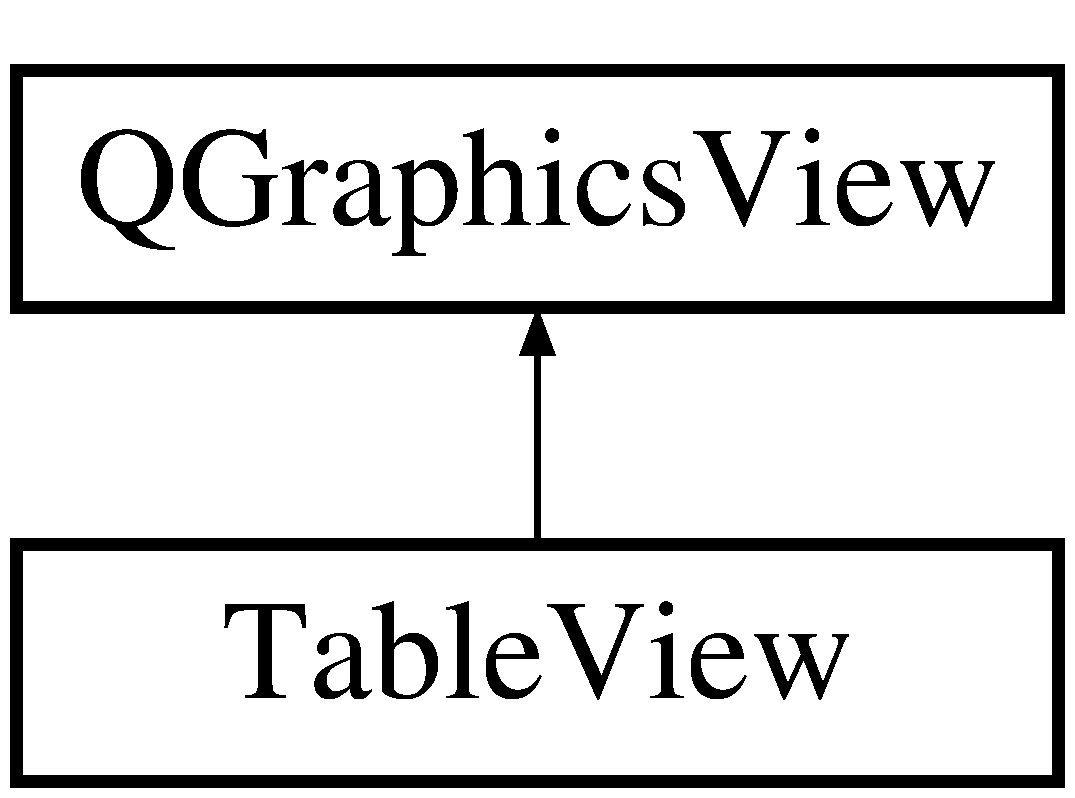
\includegraphics[height=2.000000cm]{class_table_view}
\end{center}
\end{figure}
\subsection*{Public Member Functions}
\begin{DoxyCompactItemize}
\item 
\hyperlink{class_table_view_af10efe74276fd20a864eb394492fa01e}{Table\+View} (Q\+Graphics\+Scene $\ast$table=0)
\begin{DoxyCompactList}\small\item\em \hyperlink{class_table_view}{Table\+View} constructor. \end{DoxyCompactList}\end{DoxyCompactItemize}


\subsection{Constructor \& Destructor Documentation}
\hypertarget{class_table_view_af10efe74276fd20a864eb394492fa01e}{\index{Table\+View@{Table\+View}!Table\+View@{Table\+View}}
\index{Table\+View@{Table\+View}!Table\+View@{Table\+View}}
\subsubsection[{Table\+View}]{\setlength{\rightskip}{0pt plus 5cm}Table\+View\+::\+Table\+View (
\begin{DoxyParamCaption}
\item[{Q\+Graphics\+Scene $\ast$}]{table = {\ttfamily 0}}
\end{DoxyParamCaption}
)}}\label{class_table_view_af10efe74276fd20a864eb394492fa01e}


\hyperlink{class_table_view}{Table\+View} constructor. 


\begin{DoxyParams}{Parameters}
{\em table} & pointer to the table for this tableview \\
\hline
\end{DoxyParams}


The documentation for this class was generated from the following files\+:\begin{DoxyCompactItemize}
\item 
/\+Users/khanh/\+I\+N\+F\+O3220\+\_\+\+Assignment/\+Assignment\+Three\+Base\+Two/tableview.\+h\item 
/\+Users/khanh/\+I\+N\+F\+O3220\+\_\+\+Assignment/\+Assignment\+Three\+Base\+Two/tableview.\+cpp\end{DoxyCompactItemize}

%--- End generated contents ---

% Index
\newpage
\phantomsection
\addcontentsline{toc}{chapter}{Index}
\printindex

\end{document}
